%% FEUP THESIS STYLE for LaTeX2e
%% how to use feupteses (English version)
%%
%% FEUP, JCL & JCF, 31 July 2012
%%
%% PLEASE send improvements to jlopes at fe.up.pt and to jcf at fe.up.pt
%%

%%========================================
%% Commands: pdflatex tese
%%           bibtex tese
%%           makeindex tese (only if creating an index)
%%           pdflatex tese
%% Alternative:
%%          latexmk -pdf tese.tex
%%========================================

\documentclass[11pt,a4paper,twoside,openright]{report}

%% For iso-8859-1 (latin1), comment next line and uncomment the second line
\usepackage[utf8]{inputenc}
%\usepackage[latin1]{inputenc}

%% English version

%% MIEIC options
\usepackage[mieic]{feupteses}
%\usepackage[mieic,juri]{feupteses}
%\usepackage[mieic,final]{feupteses}
%\usepackage[mieic,final,onpaper]{feupteses}

%% Additional options for feupteses.sty:
%% - onpaper: links are not shown (for paper versions)
%% - backrefs: include back references from bibliography to citation place

%% Uncomment the next lines if side by side graphics used
%\usepackage[lofdepth,lotdepth]{subfig}
%\usepackage{graphicx}
%\usepackage{float}

%% Include math package
\usepackage{mathtools}

%% Include pdf package
\usepackage{pdfpages}

%% Include toolbox package
\usepackage{etoolbox}

%% Include color package
\usepackage{color}
\definecolor{cloudwhite}{cmyk}{0,0,0,0.025}

%% Include source-code listings package
\usepackage{listings}
\lstset{ %
 language=C,                        % choose the language of the code
 basicstyle=\footnotesize\ttfamily,
 keywordstyle=\bfseries,
 numbers=left,                      % where to put the line-numbers
 numberstyle=\scriptsize\texttt,    % the size of the fonts that are used for the line-numbers
 stepnumber=1,                      % the step between two line-numbers. If it's 1 each line will be numbered
 numbersep=8pt,                     % how far the line-numbers are from the code
 frame=tb,
 float=htb,
 aboveskip=8mm,
 belowskip=4mm,
 backgroundcolor=\color{cloudwhite},
 showspaces=false,                  % show spaces adding particular underscores
 showstringspaces=false,            % underline spaces within strings
 showtabs=false,                    % show tabs within strings adding particular underscores
 tabsize=2,	                    % sets default tabsize to 2 spaces
 captionpos=b,                      % sets the caption-position to bottom
 breaklines=true,                   % sets automatic line breaking
 breakatwhitespace=false,           % sets if automatic breaks should only happen at whitespace
 escapeinside={\%*}{*)},            % if you want to add a comment within your code
 morekeywords={*,var,template,new}  % if you want to add more keywords to the set
}

%% Uncomment to create an index (at the end of the document)
%\makeindex

%% Path to the figures directory
%% TIP: use folder ``figures'' to keep all your figures
\graphicspath{{figures/}}

%%----------------------------------------
%% TIP: if you want to define more macros, use an external file to keep them
% text shorthands
%
\newcommand{\Feup}{Faculdade de Engenharia da Universidade do Porto}
\newcommand{\evm}{Eulerian Video Magnification}
\newcommand{\ica}{Independent Component Analysis}

% figure shorthand
%
\newcommand{\fig}[3][]{% position, filename, caption
\begin{figure}[#1]
  \begin{center}
    \leavevmode
    \includegraphics[width=\textwidth]{#2}
    \caption{#3}
    \label{fig:#2}
  \end{center}
\end{figure}}

% multiple line table cell
%
\newcommand{\multilinecell}[2][c]{%
  \begin{tabular}{@{}#1@{}}#2\end{tabular}}

%%----------------------------------------

%%========================================
%% Start of document
%%========================================
\begin{document}

%%----------------------------------------
%% Information about the work
%%----------------------------------------
\title{Android-based implementation of Eulerian Video Magnification for vital signs monitoring}
\author{Pedro Boloto Chambino}

%% Uncomment next line for date of submission
%\thesisdate{July 31, 2008}

%%Uncomment next line for copyright text if used
%\copyrightnotice{Name of the Author, 2008}

\supervisor{Supervisor}{Luís Teixeira}
\supervisor{Supervisor at Fraunhofer Portugal}{Luís Rosado}

%% Uncomment next line if necessary
%\supervisor{Second Supervisor}{Name of the Supervisor}

%% Uncomment committee stuff in the final version if used
%\committeetext{Approved in oral examination by the committee:}
%\committeemember{Chair}{Doctor Name of the President}
%\committeemember{External Examiner}{Doctor Name of the Examiner}
%\committeemember{Supervisor}{Doctor Name of the Supervisor}
%\signature

%% Specify cover logo (in folder ``figures'')
\logo{uporto-feup.pdf}

%% Uncomment next line for additional text  below the author's name (front page)
%\additionalfronttext{Preparação da Dissertação}

%%----------------------------------------
%% Preliminary materials
%%----------------------------------------

% remove unnecssary \include{} commands
\begin{Prolog}
  \chapter*{Abstract}

Here goes the abstract written in English.

Lorem ipsum dolor sit amet, consectetuer adipiscing elit. Sed vehicula
lorem commodo dui. Fusce mollis feugiat elit. Cum sociis natoque
penatibus et magnis dis parturient montes, nascetur ridiculus
mus. Donec eu quam. Aenean consectetuer odio quis nisi. Fusce molestie
metus sed neque. Praesent nulla. Donec quis urna. Pellentesque
hendrerit vulputate nunc. Donec id eros et leo ullamcorper
placerat. Curabitur aliquam tellus et diam. 

Ut tortor. Morbi eget elit. Maecenas nec risus. Sed ultricies. Sed
scelerisque libero faucibus sem. Nullam molestie leo quis
tellus. Donec ipsum. Nulla lobortis purus pharetra turpis. Nulla
laoreet, arcu nec hendrerit vulputate, tortor elit eleifend turpis, et
aliquam leo metus in dolor. Praesent sed nulla. Mauris ac augue. Cras
ac orci. Etiam sed urna eget nulla sodales venenatis. Donec faucibus
ante eget dui. Nam magna. Suspendisse sollicitudin est et mi. 

Fusce sed ipsum vel velit imperdiet dictum. Sed nisi purus, dapibus
ut, iaculis ac, placerat id, purus. Integer aliquet elementum
libero. Phasellus facilisis leo eget elit. Nullam nisi magna, ornare
at, aliquet et, porta id, odio. Sed volutpat tellus consectetuer
ligula. Phasellus turpis augue, malesuada et, placerat fringilla,
ornare nec, eros. Class aptent taciti sociosqu ad litora torquent per
conubia nostra, per inceptos himenaeos. Vivamus ornare quam nec sem
mattis vulputate. Nullam porta, diam nec porta mollis, orci leo
condimentum sapien, quis venenatis mi dolor a metus. Nullam
mollis. Aenean metus massa, pellentesque sit amet, sagittis eget,
tincidunt in, arcu. Vestibulum porta laoreet tortor. Nullam mollis
elit nec justo. In nulla ligula, pellentesque sit amet, consequat sed,
faucibus id, velit. Fusce purus. Quisque sagittis urna at quam. Ut eu
lacus. Maecenas tortor nibh, ultricies nec, vestibulum varius, egestas
id, sapien. 

Phasellus ullamcorper justo id risus. Nunc in leo. Mauris auctor
lectus vitae est lacinia egestas. Nulla faucibus erat sit amet lectus
varius semper. Praesent ultrices vehicula orci. Nam at metus. Aenean
eget lorem nec purus feugiat molestie. Phasellus fringilla nulla ac
risus. Aliquam elementum aliquam velit. Aenean nunc odio, lobortis id,
dictum et, rutrum ac, ipsum. 

Ut tortor. Morbi eget elit. Maecenas nec risus. Sed ultricies. Sed
scelerisque libero faucibus sem. Nullam molestie leo quis
tellus. Donec ipsum. Nulla lobortis purus pharetra turpis. Nulla
laoreet, arcu nec hendrerit vulputate, tortor elit eleifend turpis, et
aliquam leo metus in dolor. Praesent sed nulla. Mauris ac augue. Cras
ac orci. Etiam sed urna eget nulla sodales venenatis. Donec faucibus
ante eget dui. Nam magna. Suspendisse sollicitudin est et mi. 

Phasellus ullamcorper justo id risus. Nunc in leo. Mauris auctor
lectus vitae est lacinia egestas. Nulla faucibus erat sit amet lectus
varius semper. Praesent ultrices vehicula orci. Nam at metus. Aenean
eget lorem nec purus feugiat molestie. Phasellus fringilla nulla ac
risus. Aliquam elementum aliquam velit. Aenean nunc odio, lobortis id,
dictum et, rutrum ac, ipsum. 

Ut tortor. Morbi eget elit. Maecenas nec risus. Sed ultricies. Sed
scelerisque libero faucibus sem. Nullam molestie leo quis
tellus. Donec ipsum. 

\chapter*{Resumo}

O Resumo fornece ao leitor um sumário do conteúdo da dissertação.
Deverá ser breve mas conter detalhe suficiente e, uma vez que é a porta
de entrada para a dissertação, deverá dar ao leitor uma boa impressão
inicial.

Este texto inicial da dissertação é escrito no fim e resume numa
página, sem referências externas, o tema e o contexto do trabalho, a
motivação e os objectivos, as metodologias e técnicas empregues, os
principais resultados alcançados e as conclusões.

Este documento ilustra o formato a usar em dissertações na \Feup.
São dados exemplos de margens, cabeçalhos, títulos, paginação, estilos
de índices, etc. 
São ainda dados exemplos de formatação de citações, figuras e tabelas,
equações, referências cruzadas, lista de referências e índices.
%Este documento não pretende exemplificar conteúdos a usar. 
É usado texto descartável, \emph{Loren Ipsum}, para preencher a
dissertação por forma a ilustrar os formatos.

Seguem-se umas notas breves mas muito importantes sobre a versão 
provisória e a versão final do documento. 
A versão provisória, depois de verificada pelo orientador e de 
corrigida em contexto pelo autor, deve ser publicada na página 
pessoal de cada estudante/dissertação, juntamente com os dois 
resumos, em português e em inglês; deve manter a marca da água, 
assim como a numeração de linhas conforme aqui se demonstra.

A versão definitiva, a produzir somente após a defesa, em versão 
impressa (dois exemplares com capas próprias FEUP) e em versão 
eletrónica (6 CDs com "rodela" própria FEUP), deve ser limpa da marca de 
água e da numeração de linhas e deve conter a identificação, na primeira 
página, dos elementos do júri respetivo. 
Deve ainda, se for o caso, ser corrigida de acordo com as instruções 
recebidas dos elementos júri.

Lorem ipsum dolor sit amet, consectetuer adipiscing elit. Sed vehicula
lorem commodo dui. Fusce mollis feugiat elit. Cum sociis natoque
penatibus et magnis dis parturient montes, nascetur ridiculus
mus. Donec eu quam. Aenean consectetuer odio quis nisi. Fusce molestie
metus sed neque. Praesent nulla. Donec quis urna. Pellentesque
hendrerit vulputate nunc. Donec id eros et leo ullamcorper
placerat. Curabitur aliquam tellus et diam. 

Ut tortor. Morbi eget elit. Maecenas nec risus. Sed ultricies. Sed
scelerisque libero faucibus sem. Nullam molestie leo quis
tellus. Donec ipsum. Nulla lobortis purus pharetra turpis. Nulla
laoreet, arcu nec hendrerit vulputate, tortor elit eleifend turpis, et
aliquam leo metus in dolor. Praesent sed nulla. Mauris ac augue. Cras
ac orci. Etiam sed urna eget nulla sodales venenatis. Donec faucibus
ante eget dui. Nam magna. Suspendisse sollicitudin est et mi. 

Phasellus ullamcorper justo id risus. Nunc in leo. Mauris auctor
lectus vitae est lacinia egestas. Nulla faucibus erat sit amet lectus
varius semper. Praesent ultrices vehicula orci. Nam at metus. Aenean
eget lorem nec purus feugiat molestie. Phasellus fringilla nulla ac
risus. Aliquam elementum aliquam velit. Aenean nunc odio, lobortis id,
dictum et, rutrum ac, ipsum. 

Ut tortor. Morbi eget elit. Maecenas nec risus. Sed ultricies. Sed
scelerisque libero faucibus sem. Nullam molestie leo quis
tellus. Donec ipsum. 
 % the abstract
  %\chapter*{Acknowledgements}

Aliquam id dui. Nulla facilisi. Nullam ligula nunc, viverra a, iaculis
at, faucibus quis, sapien. Cum sociis natoque penatibus et magnis dis
parturient montes, nascetur ridiculus mus. Curabitur magna ligula,
ornare luctus, aliquam non, aliquet at, tortor. Donec iaculis nulla
sed eros. Sed felis. Nam lobortis libero. Pellentesque
odio. Suspendisse potenti. Morbi imperdiet rhoncus magna. Morbi
vestibulum interdum turpis. Pellentesque varius. Morbi nulla urna,
euismod in, molestie ac, placerat in, orci. 

Ut convallis. Suspendisse luctus pharetra sem. Sed sit amet mi in diam
luctus suscipit. Nulla facilisi. Integer commodo, turpis et semper
auctor, nisl ligula vestibulum erat, sed tempor lacus nibh at
turpis. Quisque vestibulum pulvinar justo. Class aptent taciti
sociosqu ad litora torquent per conubia nostra, per inceptos
himenaeos. Nam sed tellus vel tortor hendrerit pulvinar. Phasellus
eleifend, augue at mattis tincidunt, lorem lorem sodales arcu, id
volutpat risus est id neque. Phasellus egestas ante. Nam porttitor
justo sit amet urna. Suspendisse ligula nunc, mollis ac, elementum
non, venenatis ut, mauris. Mauris augue risus, tempus scelerisque,
rutrum quis, hendrerit at, nunc. Nulla posuere porta orci. Nulla dui. 

Fusce gravida placerat sem. Aenean ipsum diam, pharetra vitae, ornare
et, semper sit amet, nibh. Nam id tellus. Etiam ultrices. Praesent
gravida. Aliquam nec sapien. Morbi sagittis vulputate dolor. Donec
sapien lorem, laoreet egestas, pellentesque euismod, porta at,
sapien. Integer vitae lacus id dui convallis blandit. Mauris non
sem. Integer in velit eget lorem scelerisque vehicula. Etiam tincidunt
turpis ac nunc. Pellentesque a justo. Mauris faucibus quam id
eros. Cras pharetra. Fusce rutrum vulputate lorem. Cras pretium magna
in nisl. Integer ornare dui non pede. 

\vspace{10mm}
\flushleft{The Name of the Author}
  % the acknowledgments
  %\cleardoublepage
\thispagestyle{plain}

\vspace*{8cm}

\begin{flushright}
   \textsl{``You should be glad that bridge fell down. \\
           I was planning to build thirteen more to that same design''} \\
\vspace*{1.5cm}
           Isambard Kingdom Brunel
\end{flushright}
       % initial quotation if desired
  \cleardoublepage
  \pdfbookmark[0]{Table of Contents}{contents}
  %\setcounter{tocdepth}{1} % limit table of contents depth
  \tableofcontents
  \cleardoublepage
  \pdfbookmark[0]{List of Figures}{figures}
  \listoffigures
  \cleardoublepage
  \pdfbookmark[0]{List of Tables}{tables}
  \listoftables
  \chapter*{Abbreviations}
\chaptermark{ABBREVIATIONS}

\begin{flushleft}
\begin{tabular}{l p{0.8\linewidth}}
EVM      & \evm \\
ICA      & \ica \\
PPG      & Photo-plethysmography \\
FFT      & Fast Fourier transform \\
FPS      & Frames per second \\
JNI      & Java Native Interface \\
JVM      & Java Virtual Machine \\
OpenCV   & Open Source Computer Vision Library \\
IIR      & Infinite impulse response \\
SD       & Standard Deviation \\
\end{tabular}
\end{flushleft}
  % the list of abbreviations used
\end{Prolog}

%%----------------------------------------
%% Body
%%----------------------------------------
\StartBody

%% TIP: use a separate file for each chapter
\chapter{Introduction} \label{chap:intro}

\section*{}

% O primeiro capítulo da dissertação deve servir para apresentar o
% enquadramento e a motivação do trabalho e para identificar e
% definir os problemas que a dissertação aborda.

% Deve resumir as metodologias utilizadas no trabalho e termina
% apresentando um breve resumo de cada um dos capítulos
% posteriores.

This chapter introduces this work, by first presenting its context,
motivation, and project's objectives, on sections \ref{sec:intro:context},
\ref{sec:intro:motivation}, and \ref{sec:intro:objectives}, respectively.
Finally, section \ref{sec:intro:outline} describes the document outline.

\section{Context} \label{sec:intro:context}

% Esta secção descreve a área em que o trabalho se insere, podendo
% referir um eventual projeto de que faz parte e apresentar uma breve
% descrição da empresa onde o trabalho decorreu.

\evm{} is a method, recently presented at
\emph{SIGGRAPH}\footnote{\url{http://www.siggraph.org/}} 2012, capable of
revealing temporal variations in videos that are impossible to see
with the naked eye. Using this method, it is possible to visualize
the flow of blood as it fills the face~\cite{Wu2012Eulerian}.
Which provides enough information to assess the heart rate in a
contact-free way using a camera~\cite{Wu2012Eulerian,
Poh2010Non, Poh2011Advancements}.

The main field of this research work is \emph{image processing
and computer vision}, whose main purpose is to translate dimensional
data from the real world in the form of images into numerical
or symbolical information.

Other fields include \emph{medical applications}, \emph{software
development for mobile devices}, \emph{digital signal processing}.

This research work is an internal project of \emph{Fraunhofer
Portugal}\footnote{\url{http://www.fraunhofer.pt/}} supervised by
Luís Rosado. Fraunhofer Portugal a is non-profit private association
founded by Fraunhofer-Gesellschaft\footnote{\url{http://www.fraunhofer.de/en/about-fraunhofer/}}~\cite{Fraunhofer2013} and

\begin{quote}
  ``aims on the creation of scientific knowledge capable of
  generating added value to its clients and partners, exploring
  technology innovations oriented towards economic growth, the
  social well-being and the improvement of the quality of life of
  its end-users.''~\cite{Fraunhofer2013}
\end{quote}

\section{Motivation} \label{sec:intro:motivation}

% Apresenta a motivação e enumera os objetivos do trabalho terminando
% com um resumo das metodologias para a prossecução dos objetivos.

Due to being recently proposed, the \evm{} method implementation
has not been tested in smartphones yet.

There has been some successful effort on the assessment of vital
signs, such as, heart rate, and breathing rate, in a contact-free
way using a webcamera~\cite{Wu2012Eulerian, Poh2010Non, Poh2011Advancements},
and even a smartphone~\cite{Vitrox2013, Philips2013}.

Other similar products, which require specialist hardware and are
thus expensive, include \emph{laser Doppler}~\cite{Ulyanov1993Pulse},
\emph{microwave Doppler radar}~\cite{Greneker1997Radar}, and
\emph{thermal imaging}~\cite{Garbey2007Contact}.

Since it is a cheaper method of assessing vital signs in a
contact-free way than the above products, this research work has
potential for advancing fields, such as, \emph{telemedicine},
\emph{personal health-care}, and \emph{ambient assisting living}.

Despite the existence of very similar products by
\emph{Philips}~\cite{Philips2013} and
\emph{ViTrox Technologies}~\cite{Vitrox2013}
to the one proposed on this research work, the product to be developed
during this research work will have additional features, such as,
face tracking while assessing the heart rate, and augmented reality
to visualize the blood flow.

\section{Objectives} \label{sec:intro:objectives}

% Enumera os objetivos do trabalho terminando
% com um resumo das metodologias para a prossecução dos objetivos.

This research work goal is to test the feasibility of the
implementation of the \evm{} method on smartphones by developing
an \emph{Android} application for monitoring vital signs based on
the \evm{} method.

This application should include the following features:

\begin{itemize}
  \item heart rate detection and assessment based on the \evm{}
        method;
  \item display real-time changes, such as, the magnified blood
        flow, obtained from the \evm{} method;
  \item deal with artifacts' motion, due to, person and/or
        smartphone movement.
\end{itemize}

The application performance should then be evaluated through tests
with several individuals and the assessed heart rate compared to
the ones detected by another application~\cite{Vitrox2013, Philips2013},
and to the measurement of an electronic sphygmomanomete.

\pagebreak

\section{Outline} \label{sec:intro:outline}

% TODO rewrite outline

The rest of the document is structured as follows:

\begin{description}
  \item[Chapter~\ref{chap:sota}] introduces the concepts necessary to
        understand the presented problem. In addition, it presents
        the existing related work, and a description of the technologies
        to be used.
  \item[Chapter~\ref{chap:problem}] ...
  \item[Chapter~\ref{chap:solution}] presents the approach taken to
        solve the problem. Moreover, it introduces the testing and
        evaluation methodologies.
  \item[Chapter~\ref{chap:impl}] ...
  \item[Chapter~\ref{chap:results}] ...
  \item[Chapter~\ref{chap:conclusions}] ...
\end{description}

\chapter{State of the art} \label{chap:sota}

\section*{}

% Neste capítulo é descrito o estado da arte e são
% apresentados trabalhos relacionados para mostrar o que existe no
% mesmo domínio e quais os problemas em aberto.

% Deve deixar claro que existe uma oportunidade de desenvolvimento que
% cobre alguma falha concreta.

% O capítulo deve também efetuar uma revisão tecnológica às principais
% ferramentas utilizáveis no âmbito do projeto, justificando futuras
% escolhas.

% No final do capítulo deverá ser apresentado um resumo com as
% principais conclusões que se podem tirar.

This chapter presents several studies regarding the heart rate estimation
from a person's face captured through a simple webcam.

Section~\ref{sec:sota:photo} describe the concept that explains how the
cardiac pulse is detected from a person's face in a remote, contact-free way.

Post-processing methods, which may be applied to the retrieved signal,
are detailed on section~\ref{sec:sota:post}.

In order to estimate the heart rate, a couple of techniques are also detailed
on section~\ref{sec:sota:estimation}.

Finally, section~\ref{sec:sota:tech} reviews the main
technologies and tools used throughout this work.

\section{Photo-plethysmography} \label{sec:sota:photo}

Photo-plethysmography~(PPG) is the concept of measuring volumetric changes
of an organ optically. Its most established use is in pulse oximeters.

PPG is based on the principle that blood absorbs more light than surrounding
tissue thus variations on blood volume affect light
reflectance~\cite{Verkruysse2008Remote}.

The use of dedicated light sources and infra-red wavelengths, and contact probes
has been the norm~\cite{Ulyanov1993Pulse, Greneker1997Radar, Garbey2007Contact}.
However, recently, remote, non-contact PPG imaging has been explored. % TODO references

The method used on the article~\cite{Verkruysse2008Remote} captures the pixel
values (red, green, and blue channels) of the facial area of a previously
recorded video where volunteers were asked to minimize movements. The pixel
values within a region of interest (ROI) was then averaged for each frame.
This spatial averaging was found to significantly increase signal-to-noise
ratio. The heart rate estimation was then calculated by applying Fast Fourier
transforms and the power spectrum as explained on
section~\ref{sec:sota:estimation:power}.

The authors of~\cite{Verkruysse2008Remote} demonstrate that the fact that
the green channel features a stronger heart rate signal as compared to the
red and blue channels, is a strong evidence that the signal is due to
variations in blood volume because (oxy-) hemoglobin absorbs green light.

\section{Signal post-processing} \label{sec:sota:post}

After obtaining the raw pixel values (red, green, and blue channels), a
conjunction of the following methods may be used to extract and improve the
reflected plethysmography signal. However, each method introduces complexity
and expensive computation.

\subsection{\ica} \label{sec:sota:post:ica}

\ica{} is a special case of \emph{blind source separation} and is a relatively
new technique for uncovering independent signals from a set of observations
that are composed of linear mixtures of the underlying
sources~\cite{Comon1994Independent}.

In this case, the underlying source signal of interest is the cardiac pulse
that propagates throughout the body, which modify the path length of the
incident ambient light due to volumetric changes in the facial blood vessels
during the cardiac cycle, such that subsequent changes in amount of reflected
light indicate the timing of cardiovascular events.

By recording a video of
the facial region, the red, green, and blue~(RGB) color sensors pick up a
mixture of the reflected plethysmographic signal along with other sources of
fluctuations in light due to artifacts. Each color sensor records a mixture
of the original source signals with slightly different weights. These observed
signals from the red, green and blue color sensors are denoted by $x_{1}(t)$,
$x_{2}(t)$ and $x_{3}(t)$ respectively, which are amplitudes of the recorded
signals at time point $t$. In conventional \ica{} model the number of
recoverable sources cannot exceed the number of observations, thus three
underlying source signals were assumed, represented by $s_{1}(t)$, $s_{2}(t)$
and $s_{3}(t)$. The \ica{} model assumes that the observed signals are linear
mixtures of the sources, i.e. $x_{i}(t) = \sum_{j=1}^{3} a_{ij} s_{j}(t)$ for
each $i=1,2,3$. This can be represented compactly by the mixing equation

\begin{equation}
  x(t) = As(t)
\end{equation}

where the column vectors $x(t) = [x_{1}(t), x_{2}(t), x_{3}(t)]^{T}$,
$s(t) = [s_{1}(t), s_{2}(t), s_{3}(t)]^{T}$ and the square $3\times3$
matrix $A$ contains the mixture coefficients $a_{ij}$. The aim of \ica{} model
is to find a separating or demixing matrix $W$ that is an approximation of the
inverse of the original mixing matrix $A$ whose output

\begin{equation}
  \hat{s}(t) = Wx(t)
\end{equation}

is an estimate of the vector $s(t)$ containing the underlying source signals.
To uncover the independent sources, W must maximize the non-Gaussianity of
each source. In practice, iterative methods are used to maximize or minimize
a given cost function that measures non-Gaussianity~\cite{Poh2010Non,
Poh2011Advancements}.

\subsection{\evm} \label{sec:sota:post:evm}

\fig{evm}{Overview of the \evm{} method.}

In contrast to the \ica{} model that focus on extracting a single number,
the \evm{} uses localized spatial pooling and temporal filtering to extract
and reveal visually the signal corresponding to the cardiac pulse. This
allows for amplification and visualization of the heart rate signal at each
location on the face. This creates potential for monitoring and diagnostic
applications to medicine, i.e. the asymmetry in facial blood flow can be a
symptom of arterial problems.

Besides color amplification, the \evm{} method is also able to reveal
low-amplitude motion which may be hard or impossible for humans to see.
Previous attempts to unveil imperceptible motions in videos have been
made, such as, \cite{Liu2005Motion} which follows a \emph{Lagrangian}
perspective, as in fluid dynamics where the trajectory of particles
is tracked over time. By relying on accurate motion estimation and
additional techniques to produce good quality synthesis, such as,
motion segmentation and image in-painting, the algorithm complexity
and computation is expensive and difficult.

On the contrary, the \evm{} method is inspired by the \emph{Eulerian}
perspective, where properties of a voxel of fluid, such as pressure
and velocity, evolve over time. The approach of this method to motion
magnification is the exaggeration of motion by amplifying temporal
color changes at fixed positions, instead of, explicitly estimation
of motion.

This method approach, illustrated in figure~\ref{fig:evm}, combines
spatial and temporal processing to emphasize subtle temporal changes
in a video. First, the video sequence is decomposed into different
spatial frequency bands. Because they may exhibit different
signal-to-noise ratios, they may be magnified differently.
In the general case, the full Laplacian pyramid~\cite{Burt1983Laplacian}
may be computed. Then, temporal processing is performed on each
spatial band. The temporal processing is uniform for all spatial
bands, and for all pixels within each band. After that, the extracted
bandpass signal is magnified by a factor of $\alpha$, which can be
specified by the user, and may be attenuated automatically. Finally,
the magnified signal is added to the original and the spatial pyramid
collapsed to obtain the final output.

\subsubsection{Spatial filtering} \label{sec:sota:post:evm:spatial}

As mention before, the work of~\cite{Wu2012Eulerian} computes the full
Laplacian pyramid~\cite{Burt1983Laplacian} as a general case for spatial
filtering. Each layer of the pyramid may be magnified differently because
it may exhibit different signal-to-noise ratios, or contain spatial frequencies
for which the linear approximation used in motion magnification does not
hold~\cite[Section 3]{Wu2012Eulerian}.

Spatial filtering may also be used to significantly increases signal-to-noise
ratio, as previously mention on section~\ref{sec:sota:photo} and demonstrated
on the work of~\cite{Verkruysse2008Remote} and~\cite{Wu2012Eulerian}. Subtle
signals, such as, a person's heart rate from a video of its face, may be
enhanced this way. For this purpose the work of~\cite{Wu2012Eulerian} computes
a layer of the Gaussian pyramid which may be obtained by successively scaling
down the image by calculating the Gaussian average for each pixel.

However, for the signal of interest to be revealed, the spatial filter applied
must be large enough. Section 5 of~\cite{Wu2012Eulerian} provides an equation
to estimate the size for a spatial filter needed to reveal a signal at a
certain noise power level:

\begin{equation}
  S(\lambda) = S(r) = \sigma'^2 = k \frac{\sigma^2}{r^2}
\end{equation}

where $S(\lambda)$ represents the signal over spatial frequencies, and since
the wavelength, $\lambda$, cutoff of a spatial filter is proportional to its
radius, $r$, the signal may be represented as $S(r)$. The noise power,
$\sigma^2$, can be estimated using to the technique of~\cite{Liu2006Noise}.
Finally, because the filtered noise power level, $\sigma'^2$, is inversely
proportional to $r^2$, it is possible to solve the equation for $r$, where
$k$ is a constant that depends on the shape of the low pass filter.

\subsubsection{Temporal filtering} \label{sec:sota:post:evm:temporal}

\fig{temporal-filters}{Examples of temporal filters.}

Temporal filtering is used to extract the motions or signals to be amplified.
Thus, the filter choice is application dependent. For motion magnification,
a broad bandpass filter, such as, the butterworth filter, is preferred. A
narrow bandpass filter produces a more noise-free result for color
amplification of blood flow. An ideal bandpass filter is used
on~\cite{Wu2012Eulerian} due to its sharp cutoff frequencies. Alternatively,
for a real-time implementation low-order IIR filters can be useful for both:
color amplification and motion magnification. These filters are illustrated
on~\ref{fig:temporal-filters}.

\subsubsection{Emphasize color variations for human pulse} \label{sec:sota:evm:color}

\fig{evm-color}{Emphasis of face color changes using the \evm{} method.}

The extraction of a person's cardiac pulse using the \evm{} method
was demonstrated in~\cite{Wu2012Eulerian}. It was also presented that
using the right configuration can help extract the desired signal.
There are four steps to take when processing a video using the \evm{} method:

\begin{enumerate}
  \item select a temporal bandpass filter;
  \item select an amplification factor, $\alpha$;
  \item select a spatial frequency cutoff (specified by spatial wavelength,
        $\lambda_c$) beyond which an attenuated version of $\alpha$ is used;
  \item select the form of the attenuation for $\alpha$ —- either force
        $\alpha$ to zero for all $\lambda < \lambda_c$, or linearly scale
        $\alpha$ down to zero.
\end{enumerate}

For human pulse color variation, two temporal filters may be used, first
selecting frequencies within 0.4-4Hz, corresponding to 24-240 beats per
minute~(bpm), then a narrow band of 0.83-1Hz~(50-60 bpm) may be used,
if the extraction of the pulse rate was successful.

To emphasize the color change as much as possible, a large amplification
factor, $\alpha \approx 100$, and spatial frequency cutoff,
$\lambda_c \approx 1000$, is applied. With an attenuation of $\alpha$ to
zero for spatial wavelengths below $\lambda_c$.

The resulting output can be seen in figure~\ref{fig:evm-color}.

\subsection{Detrending} \label{sec:sota:post:detrend}

Detrending is a method of removing very large ultralow-frequency trends an
input signal without any magnitude distortion, acting as an high-pass filter.

The main advantage of the method presented on the work
of~\cite{Tarvainen2002Advanced}, compared to methods presented
in~\cite{Litvack1995Time} and~\cite{Porges1990Analysis}, is its simplicity.

The method consists of separating the input signal, $z$, into two components,
as $z = z_{stat} + z_{trend}$, where $z_{stat}$ is the nearly stationary
component, and $z_{trend}$ is the low frequency aperiodic trend component.

An estimation of the nearly stationary component, $\hat{z}_{stat}$, can
be obtained using the equation below. The detailed derivation of the equation
can be found in~\cite{Tarvainen2002Advanced}.

\begin{equation}
  \hat{z}_{stat} = (I - (I + \lambda^2 D_2^T D_2)^{-1}) z
\end{equation}

where $I$ is the identity matrix, $D_2$ is the discrete approximation of the
second order, and $\lambda$ is the regularization parameter.

\fig{detrend}{Original and detrended RR series.}

Figure~\ref{fig:detrend} presents an example of what this method is able to
achieve. The example, taken from the work of~\cite{Tarvainen2002Advanced}, uses
real RR series and the effect of the method on time and frequency domain
analysis of heart rate variability is demonstrated not to lose any useful
information.

\section{Heart rate estimation} \label{sec:sota:estimation}

In order to convert the extracted plethysmographic signal into the number
of beats per minute~(bpm), further processing must be done. Below are
highlighted two methods capable of achieving this goal.

\subsection{Power spectrum} \label{sec:sota:estimation:power}

\emph{Fourier transform} is a mathematical transform capable of converting
a function of time, $f(t)$, into a new function representing the frequency
domain of the original function.

To calculate the power spectrum, the resulting function from the
\emph{Fourier transform} is then multiplied by itself.

Since the values are captured from a video, sequence of frames, the function
of time is actually discrete, with a frequency rate equal to the video frame
rate, $FPS$.

The \emph{index}, $i$, corresponding to the maximum of the power spectrum can
then be converted into a frequency value, $F$, using the equation:

\begin{equation}
  F = \frac{i * FPS}{2 N}
\end{equation}

where $N$ is the size of the signal extracted. $F$ can then be multiplied by
$60$ to convert it to beats per minute, and have an estimation of the heart
rate from the extracted signal.

\subsection{Pulse wave detection} \label{sec:sota:estimation:pulse}

In~\cite{Nenova2010Automated}, it is presented an automated algorithm
for fast pulse wave detection. The algorithm is capable of obtaining an
estimative of the heart rate from PPG signal, as an alternative to the power
spectrum described above. Moreover, it also introduces validation to the
waveform detection by verifying its shape and timing. Below is presented a
simplified description of the algorithm. A more detailed description can be
found in~\cite{Nenova2010Automated}.

\begin{enumerate}
  \item Identification of possible peaks and foots of individual pulses
  \begin{enumerate}
    \item Maximum ($MAX$)\\
          The signal is divided into consecutive $200 ms$ time intervals and
          for every segment the absolute maximum is determined. Some of these
          maximums are rejected: if they fall below a predetermined amplitude
          threshold; or if the distance between two maximums is less than or
          equal to $200 ms$, then the lower maximum is rejected.
    \item Minimum ($MIN$)\\
          The absolute minimum is determined between every two adjacent
          maximums. A minimum is rejected, it is above a predetermined
          amplitude threshold. When a minimum is rejected, the lower-amplitude
          maximum of the two maximum adjacent to the rejected minimum is
          discarded too.
  \end{enumerate}

  \item Examination and verification of the rising edges
  \begin{enumerate}
    \item Validation of a single rising edge\\
          If a rising edge is rejected, its maximum and minimum are rejected.
          A rising edge is rejected, if its amplitude ($AMPL = MAX - MIN$) is
          lower than amplitude threshold; or its duration is lower than a
          threshold that depends on the sampling rate; or its amplitude does
          not increase smoothly.
    \item Estimation of the similarity of a rising edge to preceding and
          following rising edges accepted as valid\\
          Two rising edges are considered similar, if the amplitude of the
          lower-amplitude rising edge is greater than $50\%$ of the amplitude
          of the higher-amplitude rising edge; and if the maximum of the
          lower-amplitude rising edge is between $\pm60\%$ of the maximum of
          the higher-amplitude rising edge; and if the minimum of the
          lower-amplitude rising edge is between $\pm60\%$ of the minimum of
          the higher-amplitude rising edge; and if the duration of the shorter
          rising edge is greater then $33\%$ of the duration of the longer
          rising edge. The valid rising edges are then categorized according
          to its characteristics for the following step. The categorization
          description is suppressed for brevity and can be found
          at~\cite{Nenova2010Automated}.
    \item Verification of the current rising edge\\
          The rising edges categorized on the previous step are considered
          valid edges of a pulse wave if they fulfill at least one of the
          decision rules presented on~\cite{Nenova2010Automated} and suppressed
          for brevity.
  \end{enumerate}
\end{enumerate}

The validation process described here is important for discarding signals
which are not representative of pulse waves. Providing a way of calculating
the heart rate estimation only on valid pulse signals.

\section{Technologies} \label{sec:sota:tech}

Below are short descriptions of two of the main technologies that will be
used during this research work.

\subsection{Android SDK} \label{sec:sota:tech:android}

\emph{Android SDK} is the development kit for the \emph{Android}
platform. The \emph{Android} platform is an open source, Linux-based
operating system, primarily designed for touchscreen mobile devices,
such as, smartphones.

Because of its open source code and permissive licensing, it allows
the software to be freely modified and distributed. This have allowed
\emph{Android} to be the software of choice for technology companies
who require a low-cost, customizable, and lightweight operating system
for mobile devices and others.

\emph{Android} has also become the world's most widely used smartphone
platform with a worldwide smartphone market share of 75\%
during the third quarter of 2012~\cite{Idc2013Android}.

\emph{Android} consists of a kernel based on Linux kernel with middleware,
libraries and APIs written in C. Applications, usually, run on an application
framework which includes Java-compatible libraries based on
\emph{Apache Harmony}, an open source, free Java implementation.
\emph{Java bytecode} is then translated to run on the
\emph{Dalvik virtual machine}.

Porting existing Linux application or libraries to \emph{Android} is difficult
due to the lack of a native \emph{X Window System} and lack of support for
\emph{GNU} libraries. Support for simple C and SDL application is possible,
though, by the usage of \emph{JNI}, a programming framework that allows Java
code to call and be called by libraries written in C/C++.

\subsection{OpenCV -- Computer Vision Library} \label{sec:sota:tech:opencv}

\emph{OpenCV} is a library of programming functions mainly aimed at
real-time image processing. To support these, it also includes a
statistical machine learning library. Moreover, it is a cross-platform
and open source library that is free to use and modify under the BSD
license.

\begin{quote}
  ``OpenCV was built to provide a common infrastructure for computer
  vision applications and to accelerate the use of machine perception
  in the commercial products.''~\cite{Opencv2013About}
\end{quote}

\emph{OpenCV} is written in C/C++. There are binding for other languages,
such as, Python, Java, and even Android. However, Java and Android
implementation is recent and lacks features and stability.

\section{Chapter summary}

This chapter starts by describing the concept behind the extraction of
cardiac pulse is possible from a person's face captured through a simple video
or webcam.

It then presents several possible post-processing methods for to improve
the extraction of the actual pulse signal. These methods include:
\begin{itemize}
  \item \emph{\ica}, a method capable of uncovering independent signals from
        a set of observations that are composed of linear mixtures of the
        underlying sources;
  \item \emph{\evm}, a method inspired by the \emph{Eulerian} perspective that
        exaggerates color variations by analyzing how each pixel value
        changes over time;
  \item \emph{Detrend}, a method which removes small trends from an input
        signal without distorting its amplitude.
\end{itemize}

Then algorithms for obtaining the actual beats per minutes of the heart rate
from the signal are described:
\begin{itemize}
  \item \emph{Power spectrum}, a set of equations capable of finding the
        frequency of a signal using the \emph{Fourier transform};
  \item \emph{Pulse wave detection}, an algorithm for detecting and validating
        rising edges from a pulse signal.
\end{itemize}

Finally, important technologies for the work are described and explored:
\begin{itemize}
  \item \emph{Android}, a Linux-based operating system, primarily designed for
        touchscreen mobile devices;
  \item \emph{OpenCV}, a \emph{Computer Vision} library of programming
        functions mainly aimed at real-time image processing.
\end{itemize}

\chapter{Problem description} \label{chap:problem}

\section*{}

% Este capítulo deve começar por fazer uma apresentação detalhada do
% problema a resolver.

\section{\evm} \label{sec:problem:evm}

\section{Chapter summary}

\chapter{Implementation details} \label{chap:impl}

\section*{}

% Este capítulo pode ser dedicado à apresentação de detalhes de nível
% mais baixo relacionados com o enquadramento e implementação das
% soluções preconizadas no capítulo anterior.
% Note-se no entanto que detalhes desnecessários à compreensão do
% trabalho devem ser remetidos para anexos.

This chapter ...
% TODO

\section{Overview} \label{sec:sol:overview}

\fig{algorithm-flow}{Overview of the implemented algorithm to obtain the heart 
rate of a person from a webcam or video using the \evm{} method.}

In order to create an Android application capable of estimating a person's
heart rate, a desktop application was developed because of 
its faster implementation speed, and easier testing.
The overall algorithm was divided into several steps, illustrated in
figure~\ref{fig:algorithm-flow}, which, later, was extracted into a
library, named Pulse, to be integrated into an Android application, 
also named Pulse.
The language used to implement the desktop application and library
was C/C++. In addition, for the image processing operations, the
computer vision library, OpenCV, was used.

A short description of the overall algorithm's steps on 
figure~\ref{fig:algorithm-flow} and application workflow is as follows:

\begin{enumerate}
  \item \emph{Original frame}, read frame from device's webcam;
  \item \emph{Face detector}, detect faces in current frame and match with
        previously detected faces in order to track multiple faces.
        Each face information is then fed into the following modules:
  \begin{enumerate}
    \item \emph{\evm}, magnify detected face's rectangle;
    \item \emph{Signal noise}, verify if the signal extracted from the
          current face is too noisy. If so, that face's signal is reset
          and marked as not valid;
    \item \emph{Detrending \& Normalization}, if the current face's signal is
          not too noisy, then detrend and normalize the signal in order to
          facilitate further operations with the signal;
    \item \emph{Validate signal}, the face's signal is then validated by
          verifying its shape and timing, in a similar but simpler manner as
          found in~\cite{Nenova2010Automated}. If the signal is given as
          invalid, it is kept as valid for a couple of time, because the
          validation algorithm may miss some peaks;
    \item \emph{Calculate beats per minute}, if the current face's signal is
          valid, it is then used to estimate the person's heart rate;
  \end{enumerate}
  \item \emph{Processed frame}, the resulting frame with each magnified face
        rectangle added back to the original frame.
\end{enumerate}

Below, there are more detailed information and descriptions of the 
algorithm's steps.

\section{\evm{} implementations} \label{sec:impl:evm}

\fig{evm-flow}{Overview of the \evm{} method steps.}

This section presents the details of several different implementations of the
\evm{} method.

The first implementations, described on sections~\ref{sec:impl:evm:gdownideal},
\ref{sec:impl:evm:gdowniir} and~\ref{sec:impl:evm:lpyriir},
were developed in Java to facilitate the integration into the Android
application. However, the OpenCV Java binding was still in its early stages
which end up creating difficulties for the development. Thus, the final
implementation, on section~\ref{sec:impl:evm:final}, was implemented in C/C++,
which also reduces the number of JNI calls from the Android JVM and
increases the application performance.

The purpose of implementing multiple variants of the method was to study
how the method worked and select which spatial and temporal filters would
better fit the application goal: amplify color variation in real-time.

Figure~\ref{fig:evm-flow} shows generic steps of the method which will be
detailed on each of the following sections. The final step,
\emph{add to original frame}, however, remains the same in all
implementations. Which is when the magnified values are added back to the
original frame in order to obtain the processed frame.

\subsection{EvmGdownIdeal} \label{sec:impl:evm:gdownideal}

This was the first implementation, thus, its goal was to understand how the
method worked, and match the implementation provided, in MATLAB,
by~\cite{Wu2012Eulerian}. In addition, real-time support was implemented
by using a sliding window of $30$ frames.

\begin{description}
  \item[Resize down]\hfill\\
        This step applies a spatial filter by calculating a level of the
        Gaussian pyramid. This is achieved by looping to the desired
        level where the input to the next loop is the result from the previous
        loop, starting with the original frame. A Gaussian pyramid level is
        calculated by, first, convolving the input frame with the kernel, $K$:

        \begin{equation}
          K = \frac{1}{256}
          \begin{bmatrix}
             1 &  4 &  6 &  4 &  1 \\
             4 & 16 & 24 & 16 &  4 \\
             6 & 24 & 36 & 24 &  6 \\
             4 & 16 & 24 & 16 &  4 \\
             1 &  4 &  6 &  4 &  1 \\
          \end{bmatrix}
        \end{equation}

        and then, downsampling the frame by rejecting even rows and columns.

  \item[Temporal filter]\hfill\\
        It was used an ideal bandpass filter to remove any amplification of
        undesired frequency from the color variation of each pixel.
        To construct this ideal filter, the Fourier transform was calculated
        for each pixel over the sliding window of $30$ frames. Then,
        frequencies below $45$ and above $240$ where set to zero, and the frame
        was rebuilt using the inverse Fourier transform.

  \item[Amplification]\hfill\\
        In this step, the result of the temporal filter is multiplied by an
        $\alpha$ value. Which results in the magnification of the color
        variation selected by the temporal filter.

  \item[Resize up]\hfill\\
        This step performs the inverse operation of the \emph{resize down} step,
        where it upsamples the frame by inserting even rows and columns with
        zeros, and then, convolves the input frame with the same kernel
        multiplied by $4$. However, when the original frame is not multiple of
        two, an additional resize operation as to be done in order for the
        upsampled frame to match the original frame's size.
\end{description}

\subsection{EvmGdownIIR} \label{sec:impl:evm:gdowniir}

This implementation is very similar to the one above, but uses a different
temporal filter which does not require a sliding window of frames to support
real-time results. The filter used was an IIR bandpass filter, which was
constructed from the subtraction of two first-order lowpass IIR filters. Each
lowpass filter is computed as follows:

\begin{equation}
  L_n = L_{n-1} * (1 - \omega) + \omega * M
\end{equation}

where $M$ is the current frame, $L$ is the lowpass filter accumulator for
each frame, and $\omega$ is the cutoff frequency percentage.

The IIR temporal bandpass filter demonstrated similar results to the ideal
temporal filter used on the first implementation, without the need for
persisting a sliding window of frames, which simplifies solution and reduces
the computational power required by the device.

\subsection{EvmLpyrIIR} \label{sec:impl:evm:lpyriir}

\fig{Lpyr}{Overview of image deconstruction and reconstruction for building a
Laplacian pyramid.}

Using the same IIR temporal filter as above, this implementation uses
a different spatial filter, which, instead of, computing a level of the
Gaussian pyramid, it constructs the full Laplacian pyramid and then applies
the temporal filter to each of its bands and each band is amplified differently.

\begin{description}
  \item[Resize down]\hfill\\
        Figure~\ref{fig:Lpyr} shows the steps to decompose and reconstruct
        an image for the purpose of building a Laplacian pyramid. The
        \emph{original image} must be decomposed into two images,
        \emph{blurred} and \emph{fine}, by applying any type of spatial lowpass
        filter and scaling the image down or up by 2. In this case, a
        Gaussian filter was applied as described on steps \emph{resize down}
        and \emph{resize up} of the first implementation. Further levels of the
        pyramid can be computed by decomposing the \emph{blurred image} in the
        same manner.

  \item[Temporal filter]\hfill\\
        The temporal filter used is the IIR bandpass filter, as described above
        for the previous implementation, only this time it is applied to each
        level of the pyramid.

  \item[Amplification]\hfill\\
        The amplification method in this implementation is more complex than
        the one previously used. It is based on the implementation provided
        by~\cite{Wu2012Eulerian}. It uses a different $\alpha$ value for each
        band of spatial frequencies, which corresponds to the Laplacian pyramid
        levels. The magnification value, $\alpha$, follows the equation:

        \begin{equation}
          (1 + \alpha) \delta(t) < \frac{\lambda}{8}
        \end{equation}

        where $\delta(t)$ represents the displacement function and $\lambda$
        the spatial wavelength. Further details about this equation may be
        found on~\cite[Section 3.2]{Wu2012Eulerian}.

  \item[Resize up]\hfill\\
        This step reconstructs the \emph{original image} by iteratively
        reconstructing each \emph{blurred image} until the now processed
        \emph{original image} is reached.
\end{description}

This implementation demonstrated that by constructing a Laplacian pyramid for
the spatial filter finer motion detail would be revealed, whereas the color
variation, the property to be analyzed, was less evident.

\subsection{Performance optimized EvmGdownIIR} \label{sec:impl:evm:final}

Because the OpenCV Java binding was not complete at the time, the Java desktop
implementations were not executing fast enough for real-time processing. Thus,
a C/C++ implementation of the method that demonstrated better color variation
was developed. In addition, after studying the performance of the application,
detailed on section~\ref{sec:results:perf}, the resize operations proved to be
computationally expensive. Therefore, the \emph{Resize down} and
\emph{Resize up} steps were modified to faster resize operations that did not
alter the resulting image.

\begin{description}
  \item[Resize down]\hfill\\
        This step was changed to a single resize operation using the
        OpenCV interpolation method named \emph{area}, which produces a similar
        result to the one provided by using a Gaussian filter and downsampling
        the image.
        However, instead of, iteratively downsampling the frame multiple times,
        the resize in this step is done in only once to a predefined size.

  \item[Resize up]\hfill\\
        This step was also modified to a single resize operation using the
        linear interpolation method, which produces a good result in short
        amount of time.
\end{description}

\section{Face detection} \label{sec:impl:face}

The \emph{face detector} module uses the OpenCV object detector initially
proposed on~\cite{Viola2001Rapid} and improved on~\cite{Lienhart2002Extended}.
Which has been previously trained to detect faces.

Because object detectors are computationally expensive, therefore, in order to
improve performance, a minimum size for the face detector was set to $40\%$
of the frame width and height. In addition, since it was expected for the
person to remain still during the reading, the face detector was set to execute
only once a second.

Face tracking is simply done by matching the previous and newly detected faces
to the closest one.
\begin{itemize}
  \item If there are less newly detected faces than the previously detected
        ones, then match each new face to the nearest older face. Any older
        face that is not matched with a newly detected face is marked for
        deletion. However, it is only deleted if it fails to find a match
        on the next time the face detector executes. This measure allows the
        face detector to miss a detection of a face one time.
  \item Otherwise, if the number of newly detected faces is equal or more than
        the older faces, then match each older face to the nearest newly
        detected face. Any newly detected face that is not matched with an
        older face is then marked as a new face.
\end{itemize}

Another performance boost was achieved by only magnifying the each face
rectangle instead of the whole frame. Because of this, the face rectangle must
remain as still as possible, in order to introduce as few artifacts and noise
to the \evm{} method. To achieve this, the position and size of the face's
rectangle that is fed into the \evm{} method is interpolated between the
previous and newly detected faces, if the distance between the two, $d$,
is less than one third of the previous face's rectangle width, $w$:

\begin{equation}
  d < \frac{w}{3}
\end{equation}

And, the interpolation percentage, $r$, used is the ratio between these values:

\begin{equation}
  r = \frac{3d}{w}
\end{equation}

\section{Signal validations} \label{sec:impl:validations}

The signal validation has two phases. First, the \emph{raw} signal
obtained from the mean of a face's rectangle is checked for noise,
on step \emph{signal noise} in figure~\ref{fig:algorithm-flow}.
Then, on step \emph{validate signal}, the shape and timing of the detrended
and normalized signal is verified.

The raw signal noise is simply verified if the signal standard deviation
is higher than $50\%$ of the $\alpha$, amplification factor.

Then, each of the following operations is applied to the raw signal:
\begin{enumerate}
  \item \emph{detrend}, as in~\cite{Tarvainen2002Advanced}, also shortly
        described on section~\ref{sec:sota:post:detrend};
  \item \emph{normalization}, the normalized signal, $S'$, is obtained from
        the detrended signal, $S$, by subtracting the mean of the signal,
        $\bar{S}$, and divide it by the signal standard deviation, $\sigma$:
        \begin{equation}
          S' = \frac{S - \bar{S}}{\sigma}
        \end{equation}
  \item \emph{mean filter}, is done by convolving the signal $3$ times with
        the kernel, $K$:
        \begin{equation}
          K = \frac{1}{5 * 5}
          \begin{bmatrix}
             1 & 1 & 1 & 1 & 1 \\
             1 & 1 & 1 & 1 & 1 \\
             1 & 1 & 1 & 1 & 1 \\
             1 & 1 & 1 & 1 & 1 \\
             1 & 1 & 1 & 1 & 1 \\
          \end{bmatrix}
        \end{equation}
\end{enumerate}

Finally, the shape and timing of signal is validated by a simplification of
the fast pulse wave detection algorithm\cite{Nenova2010Automated}.
It identifies possible signal peaks by dividing the signal into consecutive
$200 ms$ time intervals and finding the absolute maximum. Some of these maximums
are rejected: if they are a boundary value of that segment; or if they fall
below a threshold, which is $60\%$ of the mean of the amplitude of the possible
identified peaks so far; or if the distance between two maximums is less than
or equal to $200 ms$, then the lower maximum is rejected.

The signal is said to be valid if:
\begin{itemize}
  \item it includes at least two peaks;
  \item the peak count is between the valid human range, between 40 and 240 bpm;
  \item the peaks' amplitude standard deviation is less than $0.5$;
  \item the standard deviation of the time interval between peaks is less
        than $0.5$;
\end{itemize}

To prevent invalidating the signal if a peak is missed or miscounted, 
the signal is kept as valid for the next 30 frames.

\section{Heart rate estimation} \label{sec:impl:estimation}

Even though the simplification of the fast pulse wave detection algorithm
presented on the previous section was capable of counting pulse wave peaks,
it would frequently miscount at least by one peak. Thus, since the period
analyzed was short, only 5 seconds at 20 frames per second, a miscounted peak
would introduce a large error to the final value.

In order to obtain the value of \emph{beats per minute} from the pulse signal, 
the method presented on section~\ref{sec:sota:estimation:power} was used
every time the signal was marked as valid.
To prevent big fluctuations, the value was averaged over the values obtained 
from the power spectrum method every 1 second.

\section{Android integration} \label{sec:impl:android}

\fig{android-flow}{Overview of the interaction between the implemented 
Android application and library.}

Due to performance, speed implementation, and easier testing, the algorithm's
library was implemented in C/C++. To integrate with the Android SDK, the 
framework \emph{Java Native Interface} was used. Because each JNI call from the 
Android SDK to the Android NDK introduces performance overhead, 
the fewer interactions the better.

The Android application workflow and interaction with the Pulse library is 
illustrated on figure~\ref{fig:android-flow}. The arrows that cross the 
modules' borders represent JNI methods' calls.

The OpenCV library is supported in the Android platform by installing 
a separate Android application which deals with selecting the appropriate 
OpenCV library for that device's architecture.

Because OpenCV for Android SDK was still in its early stage, it did not support
a couple of features which had to be implemented. Such as, switching cameras at
runtime, portrait mode, stretching frame to display container, removing
the alpha channel from the frame without introducing more overhead / operations.

\section{Chapter summary}

...
% TODO

\chapter{Results} \label{chap:results}

\section*{}

% Dependendo do volume, a avaliação do trabalho pode ser incluída no
% capítulo anterior ou pode constituir um capítulo separado.

This chapter provides the results obtained during this dissertation
and the analysis of these.

Section~\ref{sec:results:perf} reports several performance improvements
to the implemented \evm{} method and the developed algorithm to estimate
a person's heart rate.

Section~\ref{sec:results:heart} compares the measurements from the implemented
Android application, Pulse, to a sphygmomanometer, and also, to another
Android application by ViTrox that estimates a person's heart rate using
a different method.

\section{Performance} \label{sec:results:perf}

Smartphone devices have a low computational power and this was one of the
main difficulties. The first implementations of the application were not
fast enough and the implemented Android application running on a
\emph{HUAWEI MediaPad} tablet with the Android version 4.0.3 was only capturing
around 2 frames per second.

In order to improve the algorithm and application performance, metrics were
obtained using the \emph{High performance C++ Profiler}~\cite{Andrew2013High}.
This profiler was chosen because of its performance claim and easy integration
in the project.

The machine specifications on which all metrics were obtained are:

\begin{description}
  \item[Machine] MacBook Pro, 15-inch, Late 2008
  \item[Processor] 2.53 GHz Inter Core 2 Duo
  \item[Memory] 4 GB 1067 MHz DDR3
  \item[Operating System] OS X Mountain Lion
\end{description}

The input video used was the video \emph{face} found at~\cite{Wu2013Eulerian}.

On appendix~\ref{appx:perf} various tables can be found representing
several performance boosts accomplished. The unit used by the
\emph{High performance C++ Profiler} is the number of CPU cycles spent by
that operation, obtained by using the instruction
\texttt{rdtsc}~\cite{Andrew2013High}.

The main functions that needed to be optimized and analyzed are:

\begin{itemize}
  \item \texttt{Pulse::onFrame}, which is the function that detects a
        person face and estimates the heart rate for each face detected;
  \item \texttt{EvmGdownIIR::onFrame}, which is the function that
        implements the \evm{} method.
\end{itemize}

Table~\ref{tab:profile:initial} shows that these functions were spending
a big percentage of the CPU cycles, with the \texttt{Pulse} function
taking 51\% and the \evm{} method occupying 28\%.

\begin{table}[t]
  \centering
  \begin{tabular}{lrrr}
    \hline
    Operation & Calls & MCycles & Avg \\
    \hline
    Pulse::onFrame        & 301 & 15630.5432 ( 51\%) & 51.9287 \\
    EvmGdownIIR::onFrame  & 301 &  8507.6548 ( 28\%) & 28.2646 \\
    \hline
  \end{tabular}
  \caption{
    Performance metrics obtained form the initial implementation of the C/C++
    version of the desktop application. Excerpt from~\ref{pdf:profile:1}.
  }
  \label{tab:profile:initial}
\end{table}

The operations taking more CPU cycles were easily identified by the
second table on~\ref{pdf:profile:1}, also represented on
table~\ref{tab:profile:top}. These operations are:

\begin{itemize}
  \item OpenCV HighGUI module functions: \emph{wait key}, \emph{imshow},
        \emph{capture};
  \item resize operations: \emph{pyrUp}, \emph{pyrDown}, \emph{resize face box},
        and \emph{resize and draw face box back to frame};
  \item conversion operations: \emph{convert to 8 bit}, \emph{convert to float};
  \item matrix operations: \emph{add back to original frame};
  \item \emph{detect faces} operation, is the OpenCV object detector, details on
        section~\ref{sec:impl:face};
  \item \emph{detrend} operation, is the detrending method explained on
        section~\ref{sec:sota:post:detrend};
\end{itemize}

\begin{table}
  \centering
  \begin{tabular}{lrrr}
    \hline
    Operation & Calls & Self MCycles & Self Avg \\
    \hline
    wait key                                & 301 & 9892.1852 (32\%) & 32.8644 \\
    pyrUp                                   & 300 & 3472.5267 (11\%) & 11.5751 \\
    detect faces                            & 301 & 2941.3343 (10\%) & 9.7719  \\
    imshow                                  & 301 & 2555.0751 ( 8\%) & 8.4886  \\
    capture                                 & 302 & 2268.6110 ( 7\%) & 7.5120  \\
    pyrDown                                 & 301 & 1988.4146 ( 7\%) & 6.6060  \\
    convert to 8 bit                        & 300 & 1603.1581 ( 5\%) & 5.3439  \\
    detrend                                 & 301 & 1538.8180 ( 5\%) & 5.1124  \\
    resize face box                         & 301 & 1270.4278 ( 4\%) & 4.2207  \\
    resize and draw face box back to frame  & 301 & 1214.4998 ( 4\%) & 4.0349  \\
    add back to original frame              & 300 & 811.3654  ( 3\%) & 2.7046  \\
    convert to float                        & 301 & 604.0527  ( 2\%) & 2.0068  \\
    \hline
  \end{tabular}
  \caption{
    Operations taking more CPU cycles on the initial implementation of
    the C/C++ version of the desktop application when performance
    profiling was added. Excerpt from~\ref{pdf:profile:1}.
  }
  \label{tab:profile:top}
\end{table}

The first performance boost was achieved by replacing the resize operations
by faster resize methods. All together the resize operations were spending
26\% of the CPU cycles as shown by table~\ref{tab:profile:top}.
The optimizations for the operations \emph{pyrUp} and
\emph{pyrDown} are detailed on section~\ref{sec:impl:evm:final}.
The rest of the resize operations were changed to use the OpenCV
nearest neighbor interpolation method since the difference of size was small.
These optimizations reduced the total percentage of the CPU cycles
to 7\% as shown on table~\ref{tab:profile:resize}.

\begin{table}
  \centering
  \begin{tabular}{lrrr}
    \hline
    Operation & Calls & Self MCycles & Self Avg \\
    \hline
    pyrUp                                   & 300 & 583.2825 (2\%) & 1.9443 \\
    pyrDown                                 & 301 & 510.0373 (2\%) & 1.6945 \\
    resize and draw face box back to frame  & 301 & 430.7046 (2\%) & 1.4309 \\
    resize face box                         & 301 & 307.4483 (1\%) & 1.0214 \\
    \hline
  \end{tabular}
  \caption{
    Performance improvement on resize operations by using faster interpolations
    methods. Excerpt from~\ref{pdf:profile:2}.
  }
  \label{tab:profile:resize}
\end{table}

The second performance boost was accomplished by reducing the number of
executions of the OpenCV object detector. This operation was occupying
around 10\% of the CPU cycles as shown by table~\ref{tab:profile:top}.
By executing the face detection operation once every 10 frames its number
of CPU cycles was greatly reduced to 1\% as shown on
table~\ref{tab:profile:face}.

\begin{table}
  \centering
  \begin{tabular}{lrrr}
    \hline
    Operation & Calls & Self MCycles & Self Avg \\
    \hline
    detect faces &  30 & 288.2041 (1\%) & 9.6068 \\
    \hline
  \end{tabular}
  \caption{
    Performance improvement on face detection by reducing the number of times
    the OpenCV object detector was executed. Excerpt from~\ref{pdf:profile:3}.
  }
  \label{tab:profile:face}
\end{table}

A last performance boost applied to the implemented algorithm was the removal of
the resize operations \emph{resize face box} and
\emph{resize and draw face box back to frame} by modifying the \evm{} method
implemented which removed the requirement of the input image to be always of the
same size.

The result of these performance improvements are shown on
table~\ref{tab:profile:final}. With the \texttt{Pulse} function spending
only 14\% of the CPU cycles and a performance improvement of 37\%,
and the \evm{} method occupying 6\% of the CPU cycles and a performance
improvement of 22\%.

\begin{table}
  \centering
  \begin{tabular}{lrrr}
    \hline
    Operation & Calls & MCycles & Avg \\
    \hline
    Pulse::onFrame       & 300 & 4215.0788 ( 14\%) & 14.0503 \\
    EvmGdownIIR::onFrame & 287 & 1818.3953 (  6\%) &  6.3359 \\
    \hline
  \end{tabular}
  \caption{
    Final performance metrics of the main functions.
    Excerpt from~\ref{pdf:profile:4}.
  }
  \label{tab:profile:final}
\end{table}

This allowed for the implemented Android application to run at approximately
15 frames per second on the same Android device previously mentioned.

\section{Heart rate comparison} \label{sec:results:heart}

To validate the heart rate values obtained by the implemented Android
application a test was run and readings obtained to a total of 9 participants.
The procedure for the test was as follows:

\begin{enumerate}
  \item use the implemented Android application, named Pulse, to obtain an
        estimation of the person's heart rate, while at the same time
        obtain a reading from a sphygmomanometer, which also produces an
        average of the heart rate at the end, which would take
        approximately 30 seconds;
  \item then, in order to compare the results to another application,
        step one was repeated using the ViTrox application:
        \emph{What's My Heart Rate}~\cite{Vitrox2013};
  \item finally, each person was asked to do some physical exercise so
        their heart rate would increase, then step one was repeated.
\end{enumerate}

Tables~\ref{tab:heart} shows the measurements obtained by the above procedure.
In order to interpret the measurements, Bland-Altman
plots~\cite{Martin1986Statistical} were used.
The mean and standard deviation~(SD) of the differences, mean of the absolute
differences and 95\% limits of agreement ($\pm$ 1.96 SD) were calculated.

Comparing the Bland-Altman plots in figure~\ref{fig:plots:heart}, the ViTrox
application shows the best agreement against the sphygmomanometer,
figure~\ref{fig:plots:heart:vitrox:normal}; the mean bias was $1.33$ bpm
with 95\% limits of agreement $-3.56$ to $6.22$ bpm. In comparison,
the implemented application, Pulse, had a mean bias of $-12.00$ with
95\% limits of agreement $-33.13$ to $9.13$ bpm,
figure~\ref{fig:plots:heart:pulse:normal}, and after the physical exercise,
figure~\ref{fig:plots:heart:pulse:exercise}, the mean bias was $-25.89$
with 95\% limits of agreement $-51.28$ to $-0.49$ bpm.

The implemented algorithm has worse estimations with higher heart rates.
However, by picking only heart rates lower than 70 bpm according to the
sphygmomanometer, table~\ref{tab:heart:pulse:low} and
figure~\ref{fig:plots:heart:pulse:low}, the agreement between the
implemented application, Pulse, and the sphygmomanometer increases to
a mean bias of $-4.25$ with 95\% limits of agreement $-13.43$ to $4.93$ bpm.

It should be noted that the main goal of this dissertation was testing the
feasibility of implementing an \evm{}-based method on a mobile device with
the Android platform. The creation of an Android application to monitor
a person's heart rate was a simple example of the application of the
performance optimized \evm{} method developed.
Hence, the effort taken on the algorithm performance was higher than
the validation of the heart rate estimation algorithm.

% Bland-Altman values
%% pulse-normal
% mean             = -12.00
% mean + 1.96 * SD =   9.13
% mean - 1.96 * SD = -33.13
%% vitrox-normal
% mean             =   1.33
% mean + 1.96 * SD =   6.22
% mean - 1.96 * SD =  -3.56
%% pulse-after-exercise
% mean             = -25.89
% mean + 1.96 * SD =  -0.49
% mean - 1.96 * SD = -51.28
%% pulse-lower-than-70-bpm
% mean             =  -4.25
% mean + 1.96 * SD =   4.93
% mean - 1.96 * SD = -13.43

\begin{table}[p]
  \begin{subtable}{0.5\textwidth}
    \centering
    \begin{tabular}{crr}
      \hline
        Participant & \multilinecell{Pulse\\(bpm)} & \multilinecell{Sphy.\\(bpm)} \\
      \hline
        A & 55 & 57 \\
        B & 60 & 60 \\
        C & 57 & 76 \\
        D & 54 & 66 \\
        E & 47 & 75 \\
        F & 54 & 57 \\
        G & 55 & 84 \\
        H & 62 & 83 \\
        I & 56 & 59 \\
        I & 55 & 58 \\
      \hline
        Mean & 55.50 & 67.50 \\
        SD   &  3.98 & 10.97 \\
      \hline
    \end{tabular}
    \caption{
      Heart rate measurements obtained at the same time from the implemented
      Android application, Pulse, and the sphygmomanometer.
    }
    \label{tab:heart:pulse:normal}
  \end{subtable}
  ~
  \begin{subtable}{0.5\textwidth}
    \centering
    \begin{tabular}{crr}
      \hline
        Participant & \multilinecell{ViTrox\\(bpm)} & \multilinecell{Sphy.\\(bpm)} \\
      \hline
        A & 66 & 61 \\
        B & 61 & 57 \\
        C & 72 & 72 \\
        D & 65 & 63 \\
        E & 81 & 77 \\
        F & 55 & 56 \\
        G & 87 & 87 \\
        H & 79 & 82 \\
        I & 55 & 54 \\
      \hline
        Mean & 69.00 & 67.67 \\
        SD   & 11.50 & 12.19 \\
      \hline
    \end{tabular}
    \caption{
      Heart rate measurements obtained at the same time from the ViTrox
      Android application and the sphygmomanometer.
    }
    \label{tab:heart:vitrox:normal}
  \end{subtable}

  \begin{subtable}{0.5\textwidth}
    \centering
    \begin{tabular}{crr}
      \hline
        Participant & \multilinecell{Pulse\\(bpm)} & \multilinecell{Sphy.\\(bpm)} \\
      \hline
        A & 54 &  87 \\
        B & 66 &  65 \\
        C & 57 &  98 \\
        D & 48 &  71 \\
        E & 64 &  84 \\
        F & 51 &  63 \\
        G & 69 & 102 \\
        H & 66 & 105 \\
        I & 47 &  80 \\
      \hline
        Mean & 58.00 & 83.89\\
        SD   &  8.46 & 15.64 \\
      \hline
    \end{tabular}
    \caption{
      Heart rate measurements obtained at the same time from the implemented
      Android application, Pulse, and the sphygmomanometer, after physical
      exercise.
    }
    \label{tab:heart:pulse:exercise}
  \end{subtable}
  ~
  \begin{subtable}{0.5\textwidth}
    \centering
    \begin{tabular}{crr}
      \hline
        Participant & \multilinecell{Pulse\\(bpm)} & \multilinecell{Sphy.\\(bpm)} \\
      \hline
        A & 55 & 57 \\
        B & 60 & 60 \\
        B & 66 & 65 \\
        D & 54 & 66 \\
        F & 54 & 57 \\
        F & 51 & 63 \\
        I & 56 & 59 \\
        I & 55 & 58 \\
      \hline
        Mean & 56.38 & 60.63 \\
        SD   &  4.63 &  3.58 \\
      \hline
    \end{tabular}
    \caption{
      Selection of heart rate measurements obtained from the Pulse application
      with an heart rate of 70 bpm or lower according to the sphygmomanometer.
    }
    \label{tab:heart:pulse:low}
  \end{subtable}

  \caption{
    Heart rate measurements obtained following the procedure described
    from a sphygmomanometer and an Android application:
    either Pulse, (a), (c), (d), which is the developed application,
    or the ViTrox application, (b).
  }
  \label{tab:heart}
\end{table}

\begin{figure}[p]
  \begin{subfigure}{0.5\textwidth}
    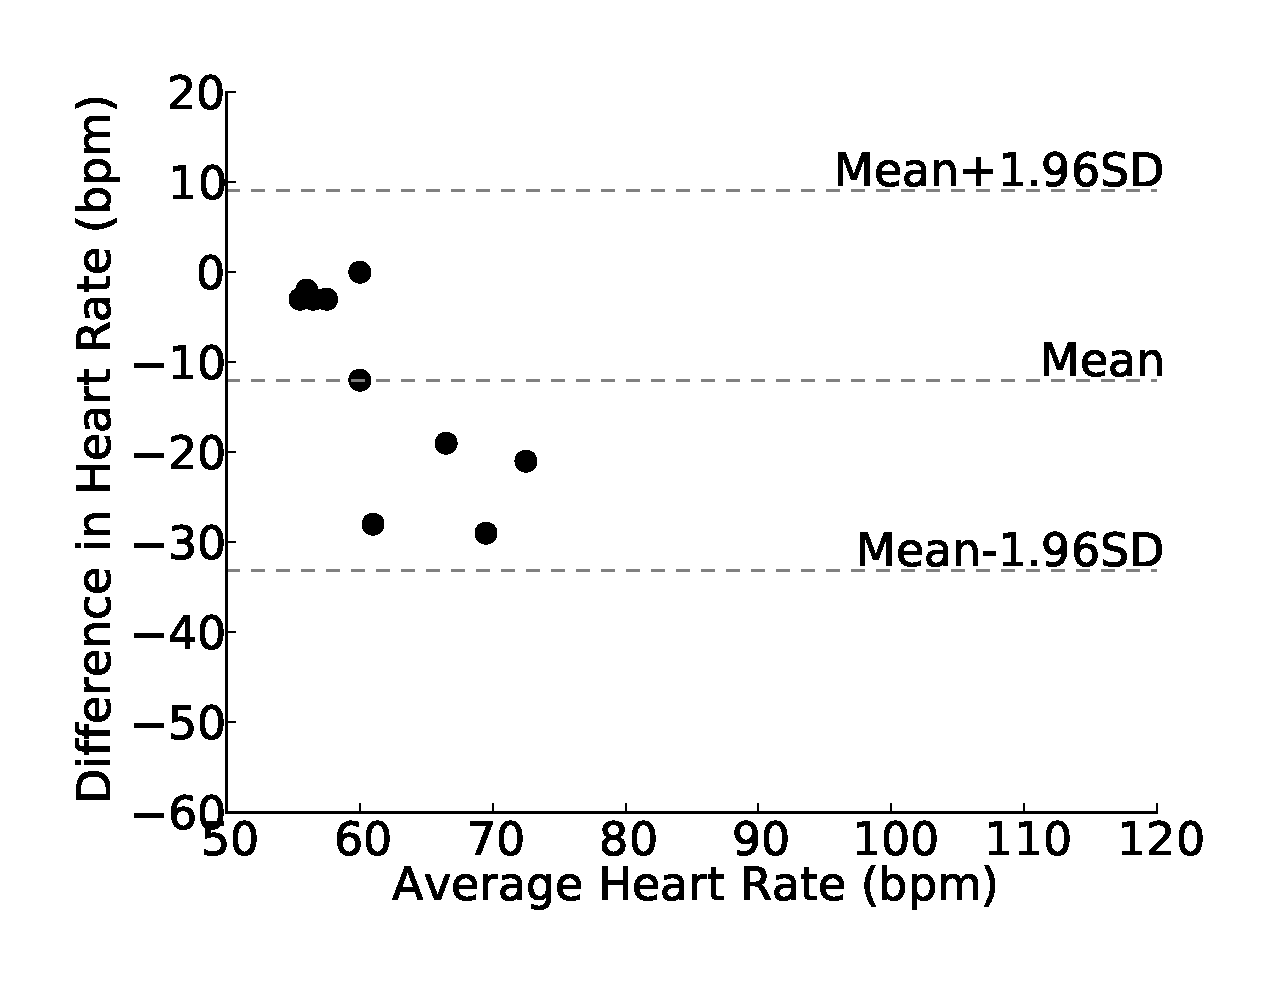
\includegraphics[width=\textwidth]{plots/pulse-normal}
    \caption{Pulse and sphygmomanometer.}
    \label{fig:plots:heart:pulse:normal}
  \end{subfigure}
  ~
  \begin{subfigure}{0.5\textwidth}
    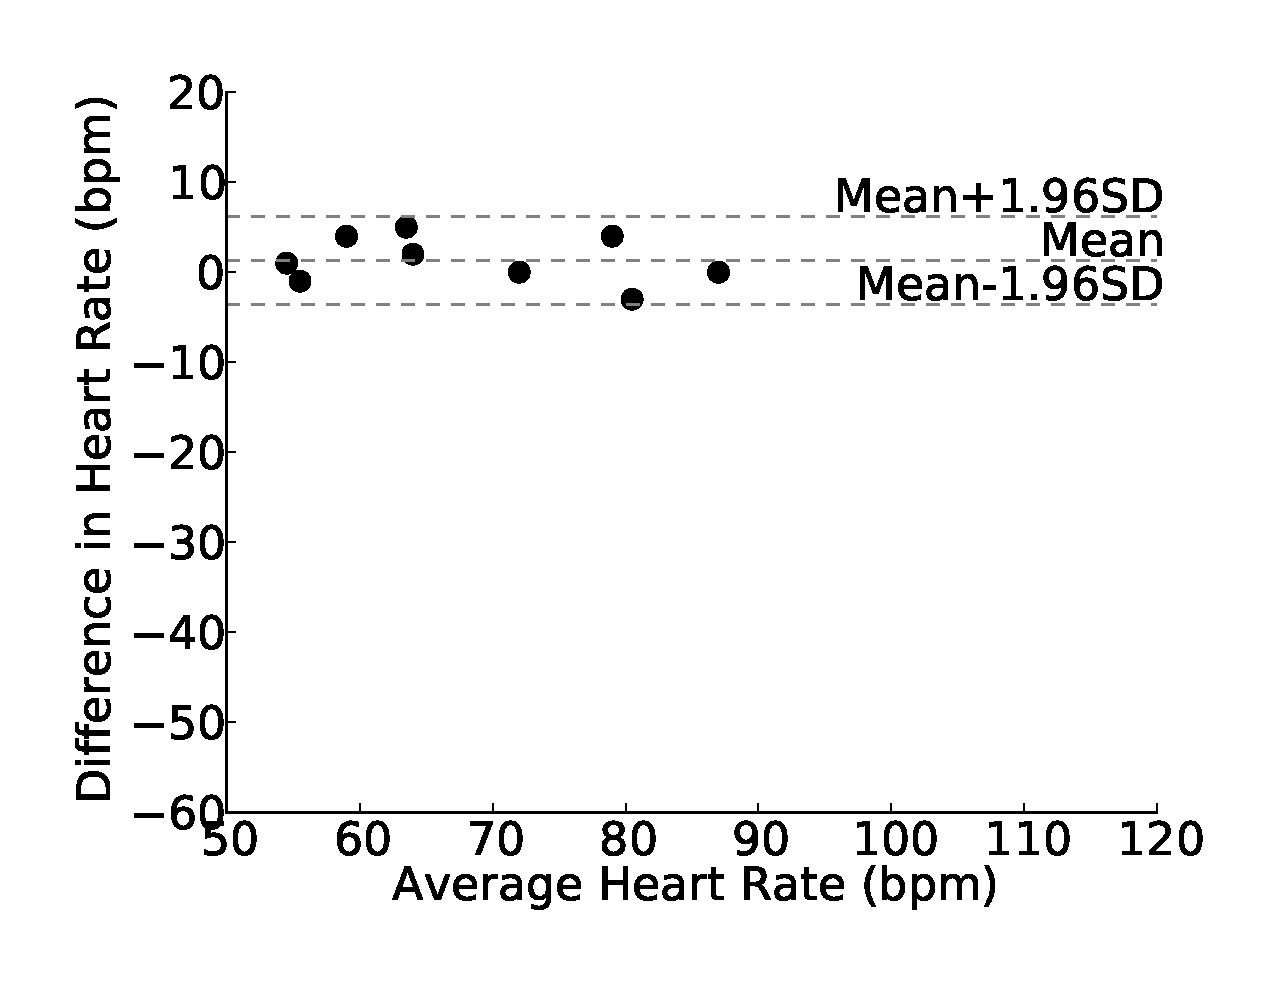
\includegraphics[width=\textwidth]{plots/vitrox-normal}
    \caption{ViTrox and sphygmomanometer.}
    \label{fig:plots:heart:vitrox:normal}
  \end{subfigure}

  \begin{subfigure}{0.5\textwidth}
    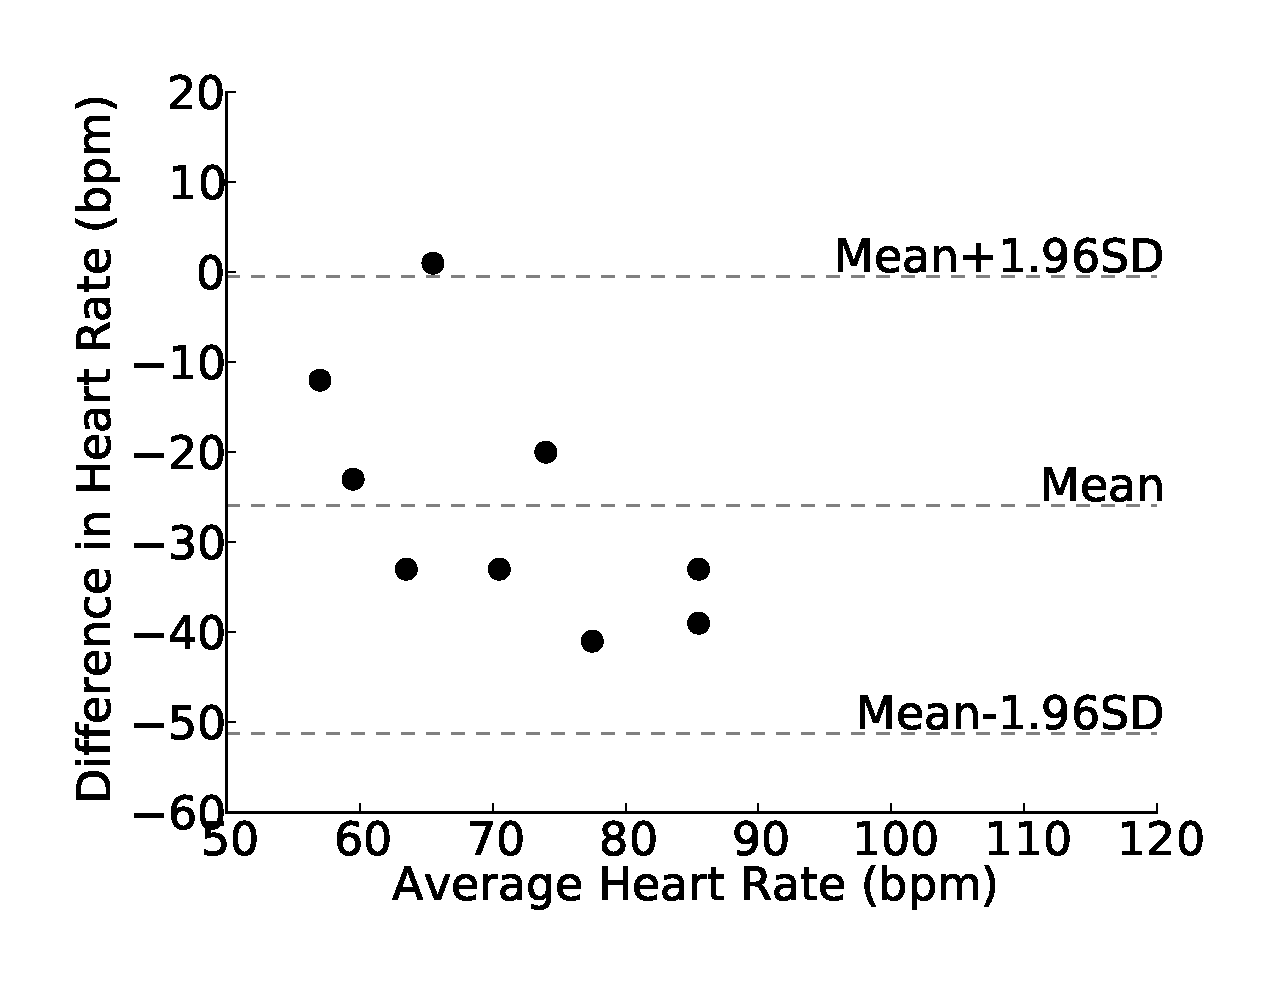
\includegraphics[width=\textwidth]{plots/pulse-after-exercise}
    \caption{Pulse and sphygmomanometer, after physical exercise.}
    \label{fig:plots:heart:pulse:exercise}
  \end{subfigure}
  ~
  \begin{subfigure}{0.5\textwidth}
    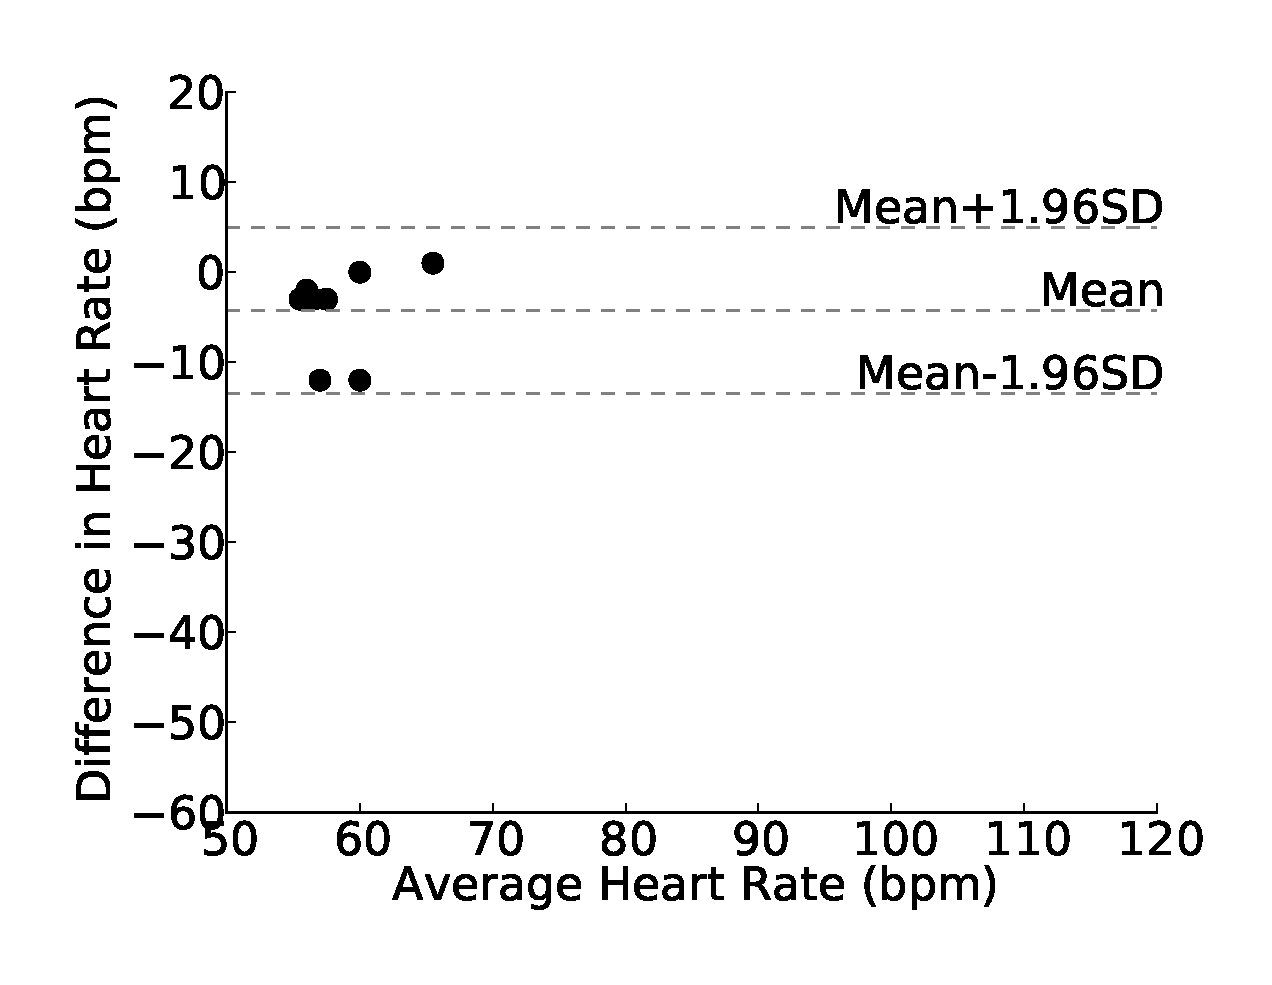
\includegraphics[width=\textwidth]{plots/pulse-lower-than-70-bpm}
    \caption{
      Pulse and sphygmomanometer, only measurements with an heart rate lower
      than 70 bpm according to the sphygmomanometer.
    }
    \label{fig:plots:heart:pulse:low}
  \end{subfigure}

  \caption{
    Bland-Altman plots demonstrating the agreement between the heart rate
    measurements obtained from a sphygmomanometer and an Android application:
    either Pulse, (a), (c), (d), which is the developed application,
    or the ViTrox application, (b).
  }
  \label{fig:plots:heart}
\end{figure}

\section{Chapter summary}

In this chapter, the performance optimizations of the algorithm and application
along with its metrics are presented. From a basic, real-time
implementation of the \evm{} method to an optimized version capable of
executing on an Android device at a reasonable rate of 15 frames per second
and a performance improvement of 22\%.

In addition, the heart rate estimations obtained using the
implemented Android application, Pulse, were compared to readings
from a sphygmomanometer and another Android application from
\emph{ViTrox Technologies}. Using Bland-Altman plots the best agreement
was between the Vitrox application and the sphygmomanometer, where the mean
bias was $1.33$ bpm with 95\% limits of agreement $-3.56$ to $6.22$ bpm.
Followed by the Pulse application and the sphygmomanometer, when the
beats per minute was lower than 70 according to the sphygmomanometer, with a
mean bias of $-4.25$ with 95\% limits of agreement $-13.43$ to $4.93$ bpm.

\chapter{Conclusions} \label{chap:conclusions}

\section*{}

% Deve ser apresentado um resumo do trabalho realizado e apreciada a
% satisfação dos objetivos do trabalho, uma lista de contribuições
% principais do trabalho e as direções para trabalho futuro.

% A escrita deste capítulo deve ser orientada para a total compreensão
% do trabalho, tendo em atenção que, depois de ler o Resumo e a
% Introdução, a maioria dos leitores passará à leitura deste capítulo de
% conclusões e recomendações para trabalho futuro.

\section{Objective satisfaction} \label{sec:conclusions:objectives}

\section{Future work} \label{sec:conclusions:future}

% TODO


%%----------------------------------------
%% Final materials
%%----------------------------------------

%% Bibliography
%% Comment the next command if BibTeX file not used
%% bibliography is in ``myrefs.bib''
\PrintBib{myrefs}

%% comment next 2 commands if numbered appendices are not used
\appendix
\chapter{Performance metrics} \label{appx:perf}

This appendix presents performance metrics for the desktop application
implemented using the \emph{High performance C++ Profiler}. For further
details refer to section~\ref{sec:results:perf}.

Each performance metric contains two tables. The first is ordered by
function structure and total cycles the CPU spent on that function. The second
table is ordered by self cycles, which represents the total cycles the CPU spent
on that function minus the total cycles the CPU spent on the children functions.

The short descriptions of the performance metrics and the page number
where each can be found follows:

\newcommand{\profile}[1]{% index
  \ifnumequal{#1}{1}{
    Initial performance metrics.
  }{}
  \ifnumequal{#1}{2}{
    Performance metrics using faster resize operations.
  }{}
  \ifnumequal{#1}{3}{
    Performance metrics when face detection was executed every 10 frames
    instead of every frame.
  }{}
  \ifnumequal{#1}{4}{
    Performance metrics with no \emph{resize face box} and
    \emph{resize and draw face box back to frame} operations since the
    \emph{EvmGdownIIR} implementation always resizes to a predefined size.
  }{}
}

\begin{description}
  \item[Appendix \ref{pdf:profile:1} on page~\pageref{pdf:profile:1}]\hfill\\\profile{1}
  \item[Appendix \ref{pdf:profile:2} on page~\pageref{pdf:profile:2}]\hfill\\\profile{2}
  \item[Appendix \ref{pdf:profile:3} on page~\pageref{pdf:profile:3}]\hfill\\\profile{3}
  \item[Appendix \ref{pdf:profile:4} on page~\pageref{pdf:profile:4}]\hfill\\\profile{4}
\end{description}

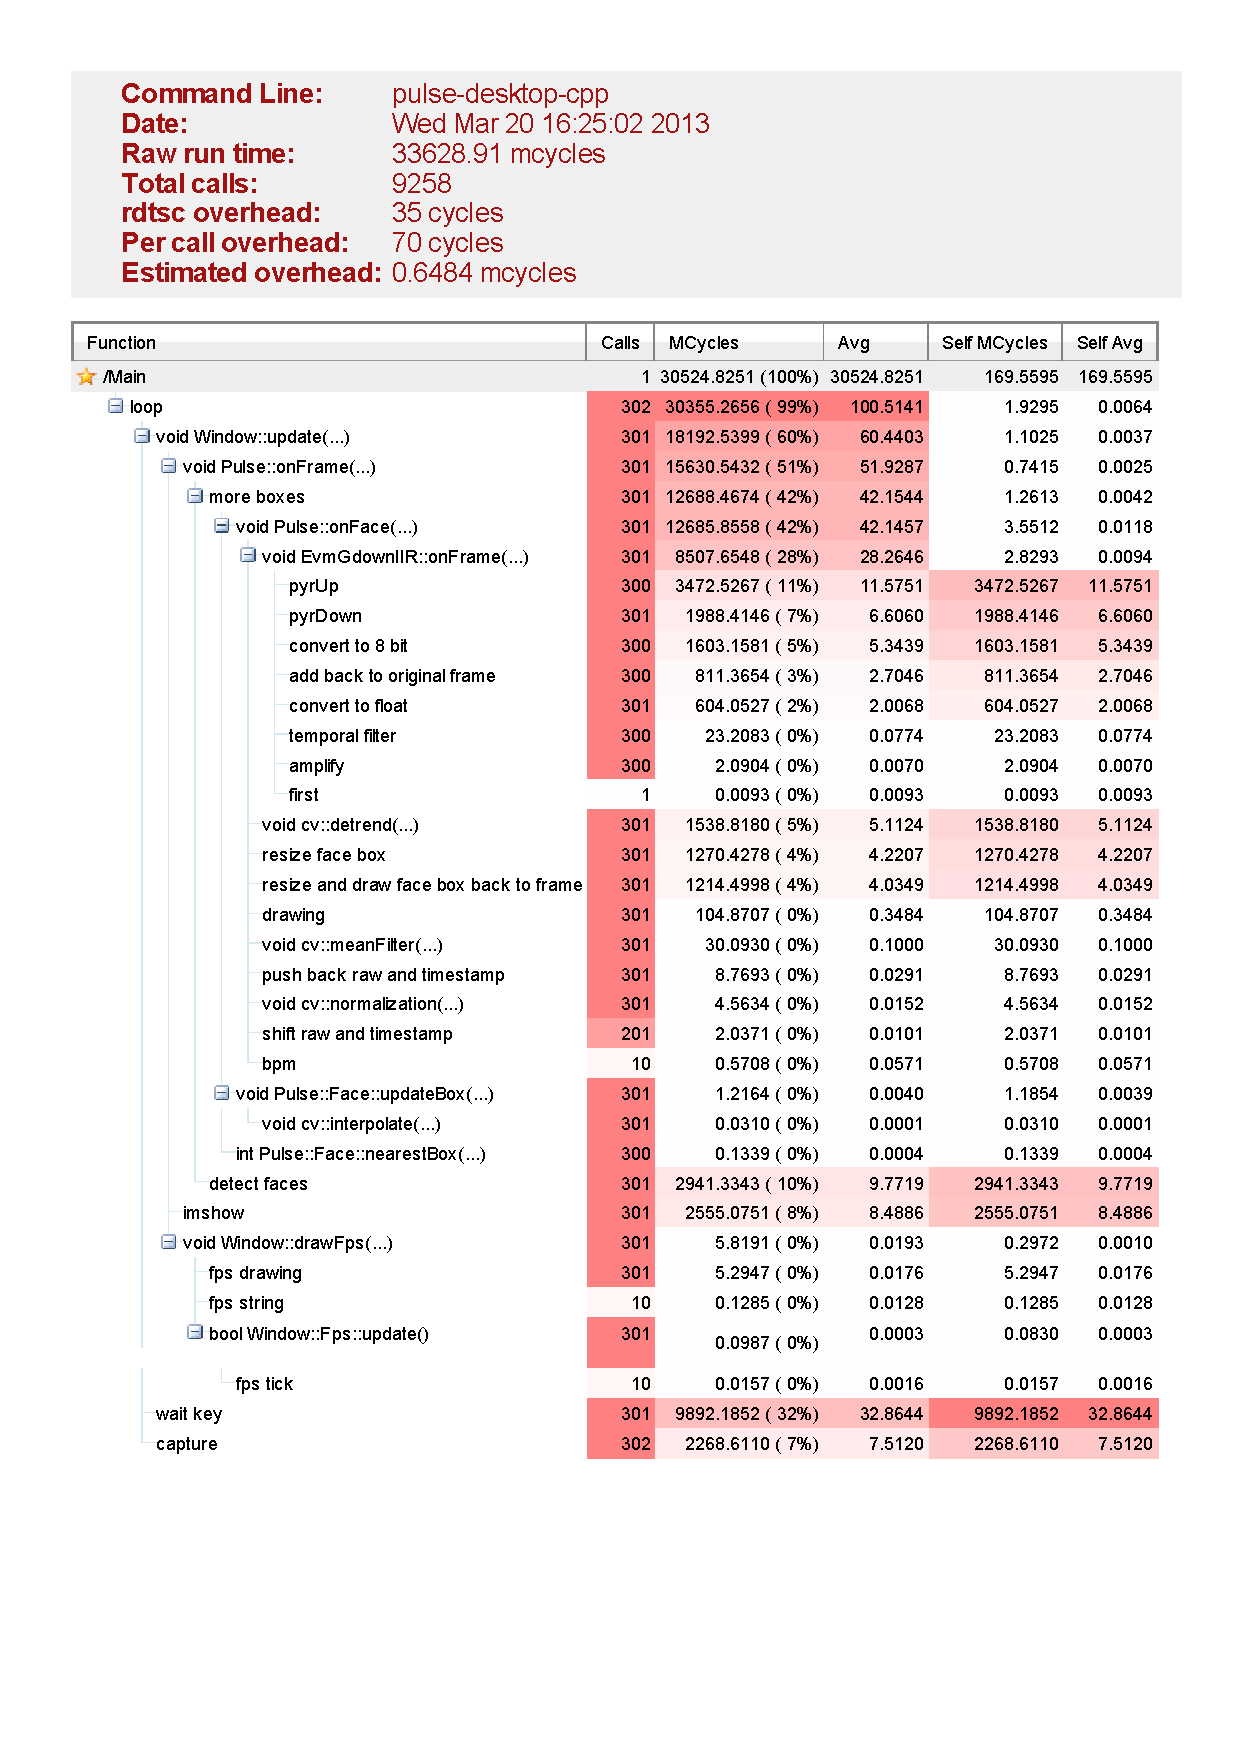
\includepdf[
  pages=-,
  pagecommand={\thispagestyle{plain}},
  addtolist={1, table, \profile{1}, pdf:profile:1}
]{profile/1}

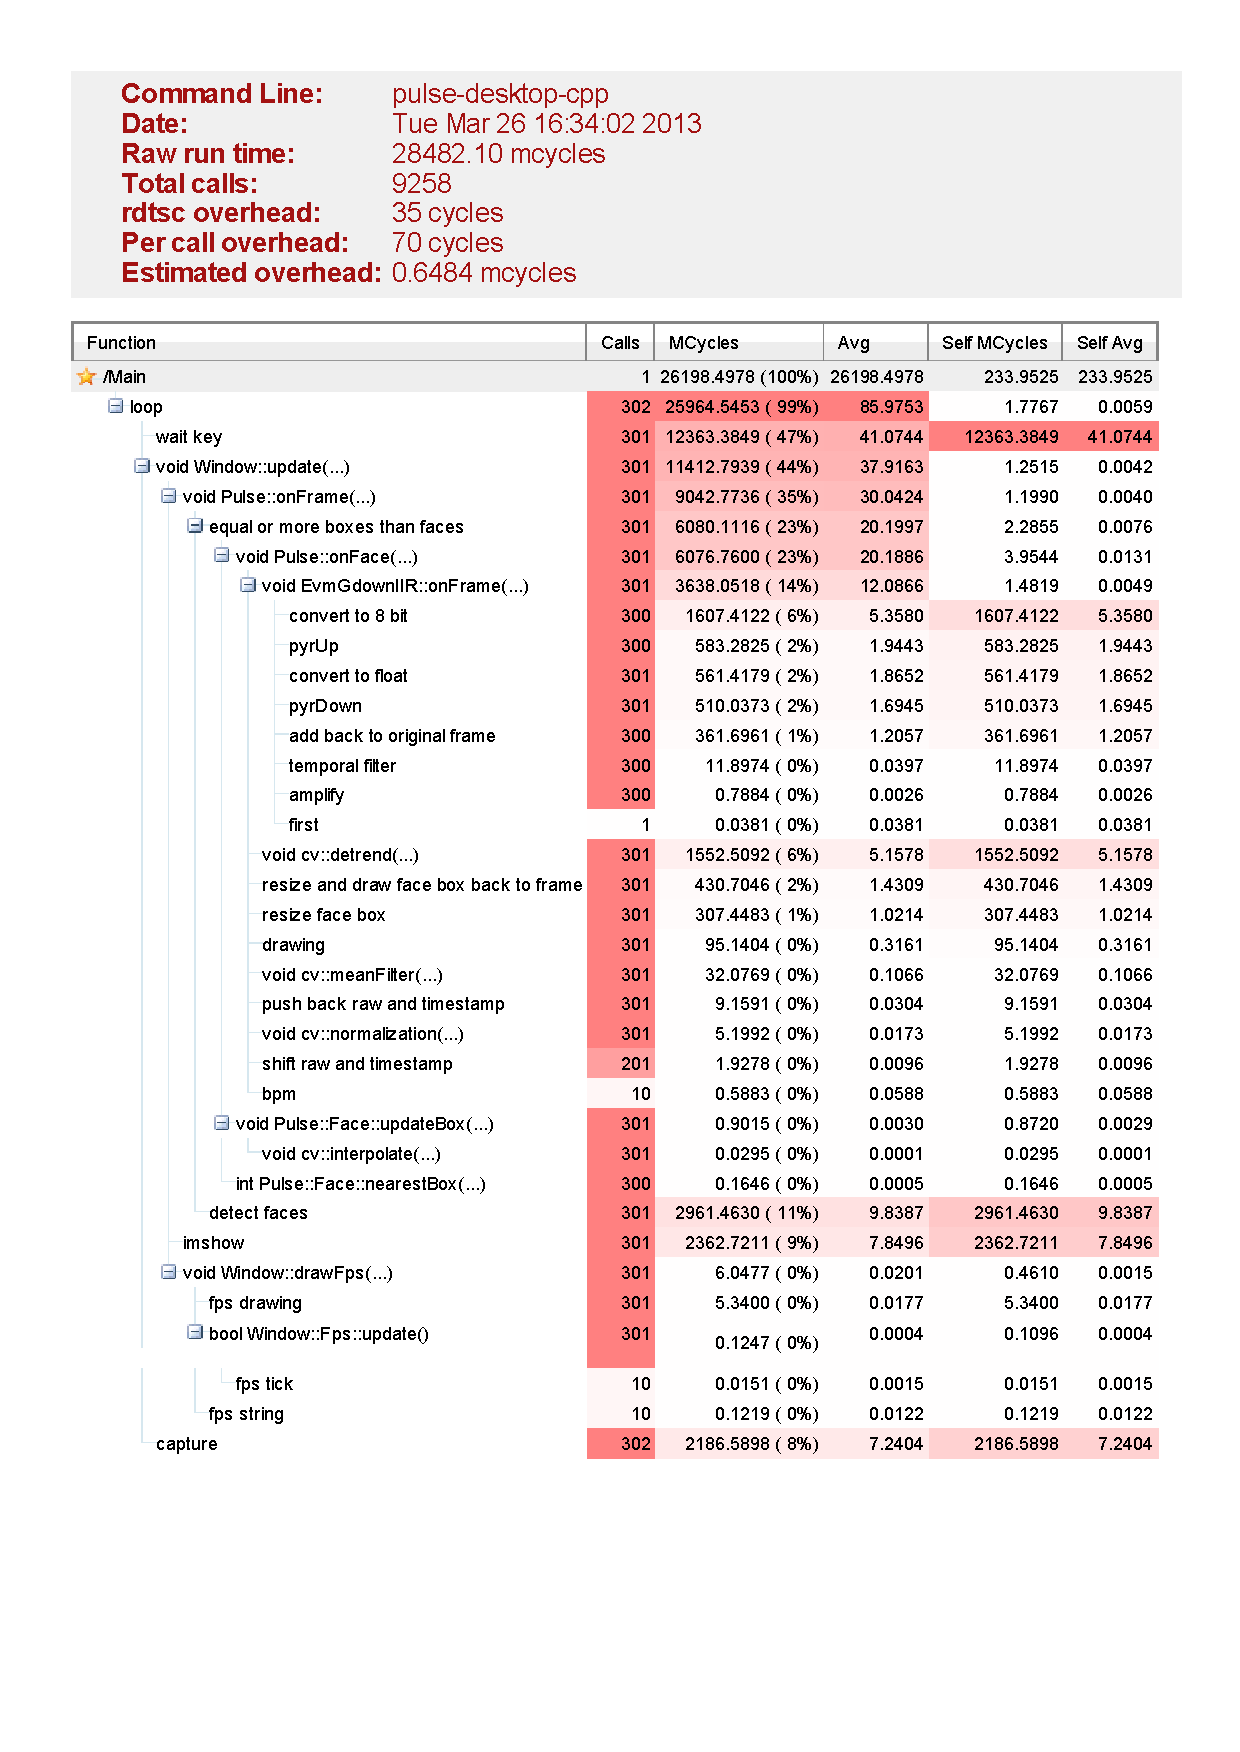
\includepdf[
  pages=-,
  pagecommand={\thispagestyle{plain}},
  addtolist={1, table, \profile{2}, pdf:profile:2}
]{profile/2}

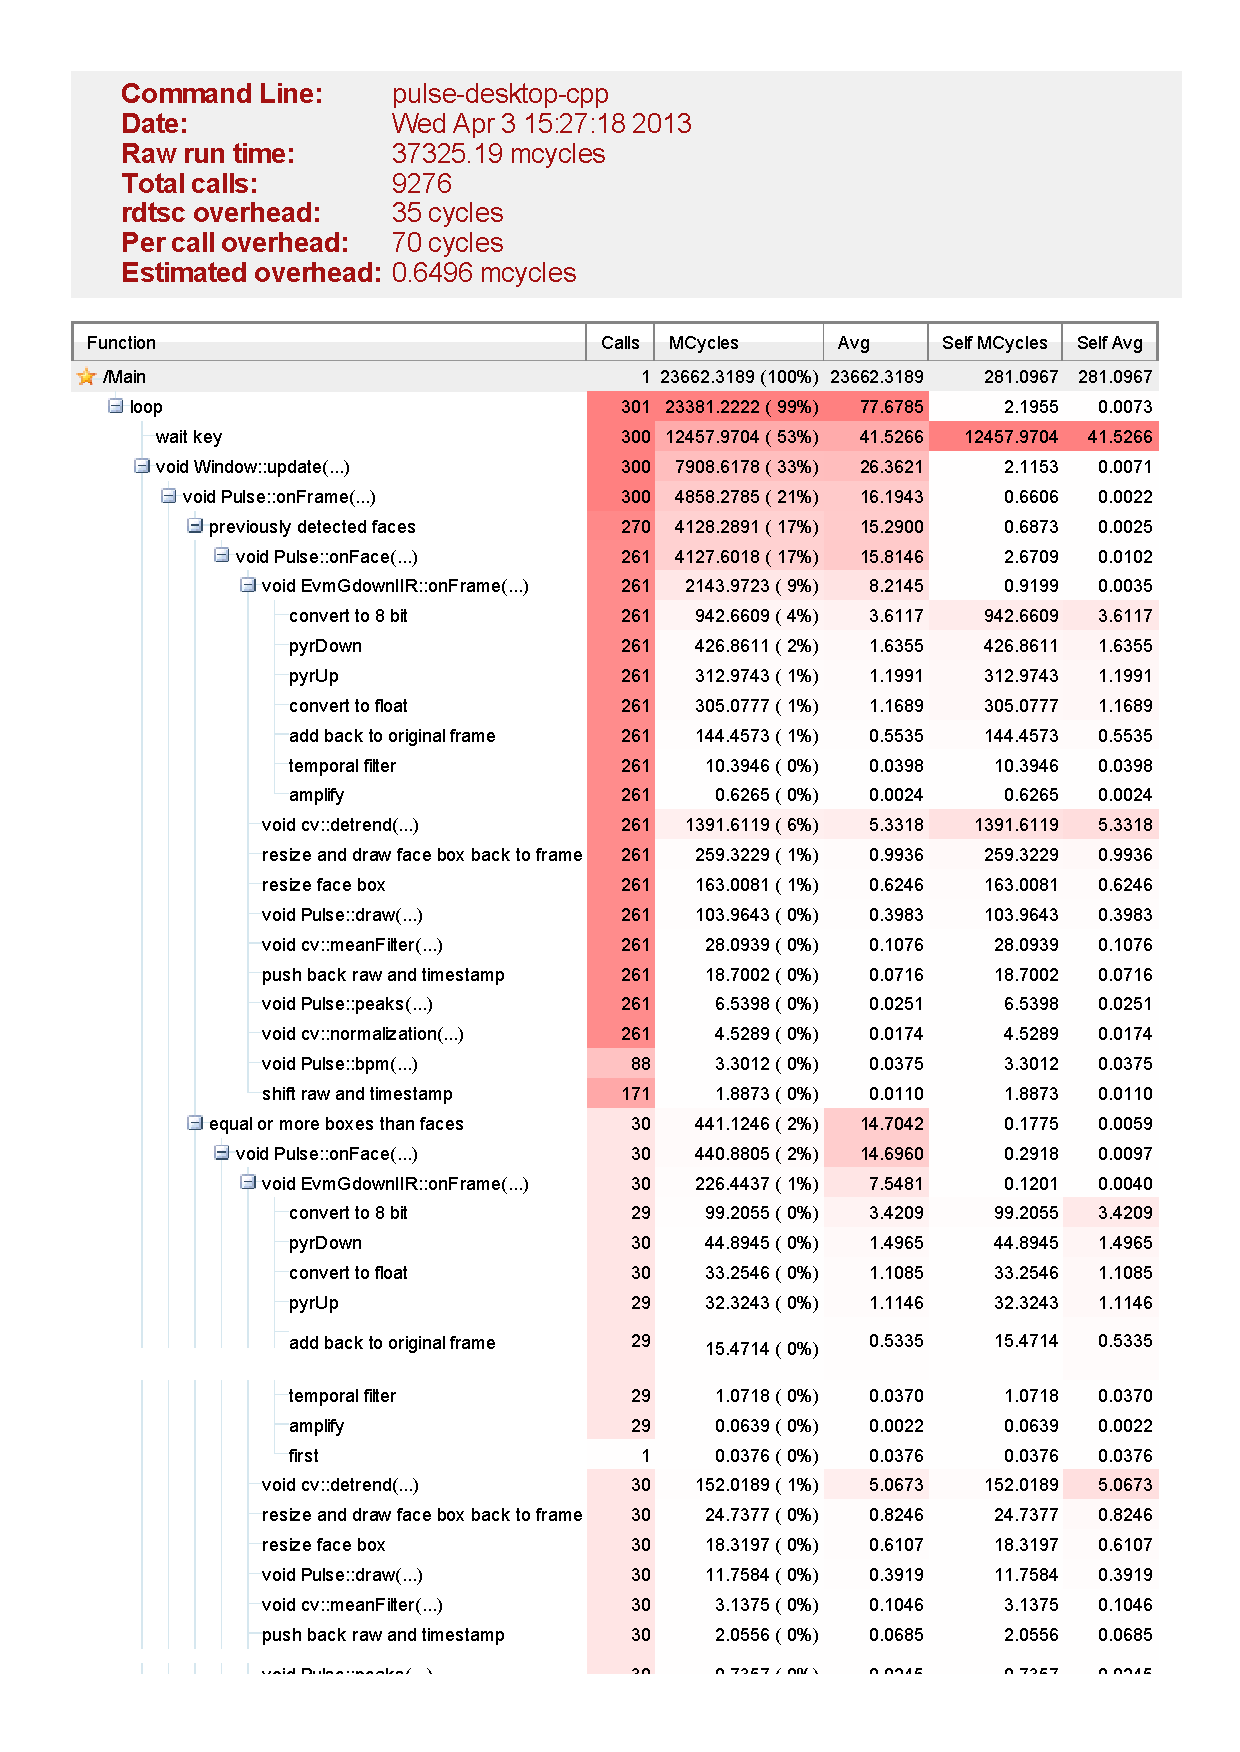
\includepdf[
  pages=-,
  pagecommand={\thispagestyle{plain}},
  addtolist={1, table, \profile{3}, pdf:profile:3}
]{profile/3}

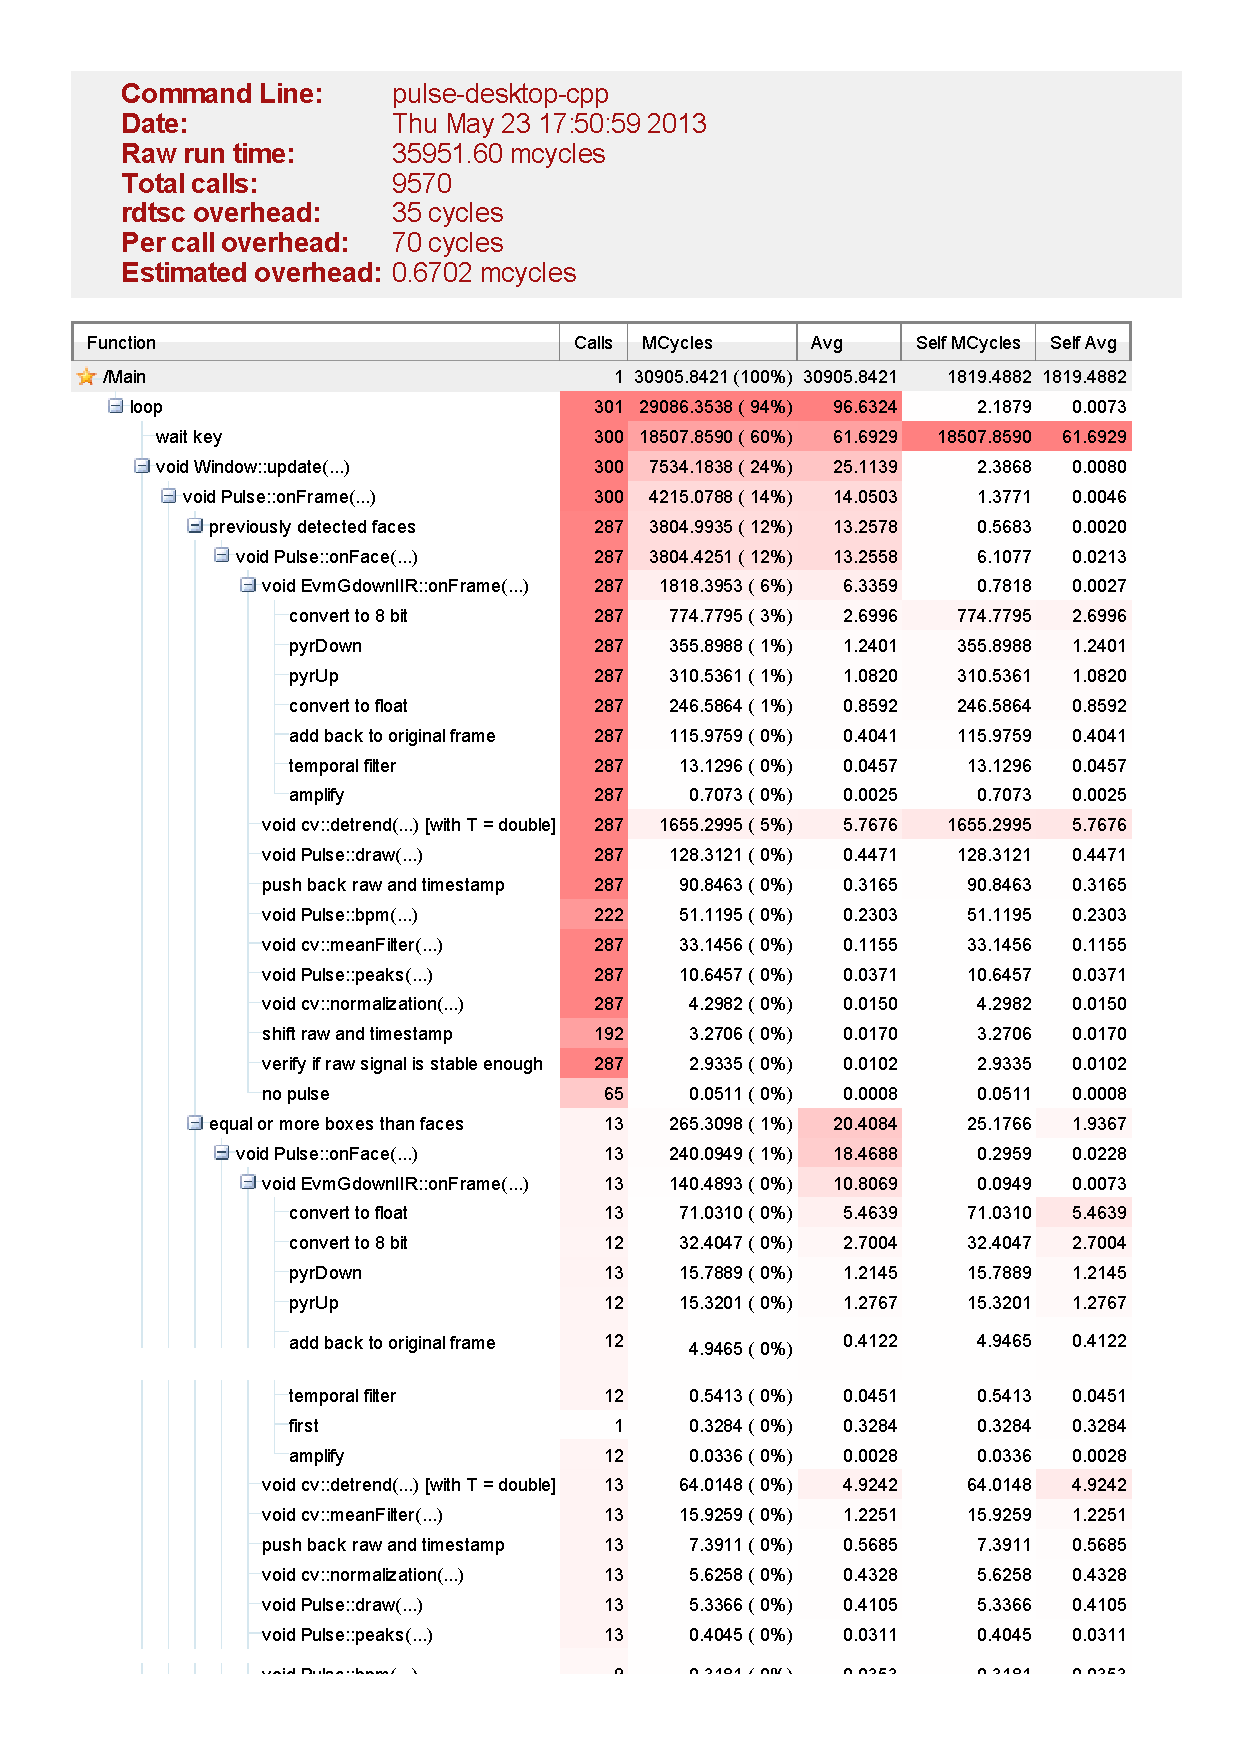
\includepdf[
  pages=-,
  pagecommand={\thispagestyle{plain}},
  addtolist={1, table, \profile{4}, pdf:profile:4}
]{profile/4}


%% Index
%% Uncomment next command if index is required
%% don't forget to run ``makeindex mieic-en'' command
%\PrintIndex

\end{document}
